\documentclass{article}
\usepackage{graphicx} 
\usepackage{amsmath, amsfonts, amssymb, amsthm}
\usepackage{tikz}
\usepackage{float}
\usepackage{hyperref}
\usepackage{caption}
\usepackage{subcaption}
%This two lines make it so that each section starts in a new page, in case we want to use it
%\usepackage{titlesec}
%\newcommand{\sectionbreak}{\clearpage}

\usetikzlibrary{graphs}
\usepackage[demo]{graphicx}

% just took these from the presentation. might have some errors, idk how this stuff works
\usepackage{tikz}
\usepackage{pgfplots}
\pgfplotsset{compat = newest}
\usetikzlibrary{matrix}
\usepackage[dvipsnames]{xcolor}

\usepackage[shortlabels]{enumitem}


% copypasted from 
% https://www.dickimawbooks.com/latex/thesis/html/amsthm.html
\theoremstyle{plain}
\newtheorem{theorem}{Theorem}
\newtheorem{defn}{Definition}
\newtheorem{lemma}{Lemma}
\newtheorem*{minidef*}{}
\newtheorem{corollary}{Corollary}

\theoremstyle{definition}
\newtheorem{exmp}{Example}[section]


\theoremstyle{remark}
\newtheorem*{note}{Note}
\newtheorem{remark}{Remark}


\usepackage{verbatim}
\usepackage{tabularx}
\usepackage{indentfirst} % Indent first paragraph in each section
\usepackage[a4paper, total={6in, 8.1in}]{geometry}
\usepackage{setspace}


\newcommand{\mat}{\text{Mat}}
\newcommand{\cl}{\mathrm{cl}}
\newcommand{\caf}{\mathcal{F}}
\newcommand{\rank}{\text{r}}
\newcommand{\ev}{\mathrm{ev}}

\onehalfspacing

% Equations should be numbered per section
\numberwithin{equation}{section}




    \title{ {
\includegraphics[scale=0.5]{rug_logo.png}}\\
    \vspace{2cm}
    {Cryptomorphic Descriptions of Matroids} ,
    }
    \author{Adriel Matei, Béla Schneider, Javier Vela Castro, Juš Kocutar}




\begin{document}


\maketitle


\newpage

\tableofcontents

\newpage
\section{Introduction}
\subsection{(In)dependence}

In english language, two peolpe, objects or concepts are dependent on each other if both in some way influence one another. Two things being independent from each other then means that they in no way can affect eachother. 

In mathematics there are many concepts where we can use these two words to describe certain phenomena, most notably, linear algebra. In linear algebra, a set of vectors is linearly dependent if you can write one of its vectors as a linear combination of the others. Using the word dependent here makes sense, because if you can use all others to build that one vector, then that vertor does not really stand on its own. An equivalent and more general definition is:
$$ \{v_1,v_2,\dots,v_n\} \text{ is linearly dependent if} $$ $$ \text{there exists } a_1,a_2,\dots,a_n \in \mathbb{R} \text{ not all zero, such that } a_1v_1+a_2v_2+\dots +a_nv_n = 0$$
For linear independence we have the negation, which is:
$$ \{v_1,v_2,\dots,v_n\} \text{ is linearly independent if } $$ $$ a_1v_1+a_2v_2+\dots+a_nv_n=0 \text{ implies that } a_1=a_2=\dots=a_n=0 $$

There are many more fields that have this concept of (in)dependence present in some way. To relate these with another we will abstract the concept of (in)dependence into mere sets that follow certain rules. It turns out that by doing this we can find independence in places that do not even use the terms (in)dependence, most notably, graph theory.

TODO: give an intuitive explaination on why cycles in graphs are somehow 'dependent'





\newpage

\subsection{Matroids}

A matroid is a structure that abstracts the notion of independence. To construct a matroid we first start with a ground set that is finite. We do not want to work with infinite sets, because that causes lots of problems. Next, we construct a set of subsets of the ground set, following a couple of rules. Usually, this would be the set of independent sets. However, it turns out that there are many surprisingly equivalent (cryptomorphic) ways of defining a matroid, such as:
\begin{itemize}
    \item Independent sets
    \item Bases
    \item Circuits
    \item Rank function
    \item Closure operator
    \item Flats
\end{itemize}

There are many more cryptomorphic ways to define a matroid, but the ones listed will be covered in this article. Each of these mathematical objects has two to four axioms that uniquely determine it as the object characterizing a matroid. To show the cryptomorphism, we will have to prove a certain equivalence each time. All of this will help us gain a deeper insight into the concept of dependence and independence.



\section{Elementary Definitions}

\subsection{Independent sets}

We will begin with the first possible way of defining what a \textit{matroid} is. This way is arguably the simplest one because the properties are intuitive and not hard to visualize. When speaking about matroids we will always deal with finite sets, and the way we obtain a matroid from a finite set is to select some special selection of its subsets.  these special sets correspond to the \textit{independent} sets, and should obey some distinctive properties. This idea is precisely what the following definition is about.

\begin{defn}
    Let $E$ be a finite set, possibly empty and $\mathcal{I}$ a collection of subsets of $E$ (i.e. some subset of the power set $2^E$ of E). We call the ordered pair $M = (E, \mathcal{I})$ a matroid if the following three properties are satisfied

    \begin{enumerate}
        \item We have $\emptyset \in \mathcal{I}$.
        
        \item If $I \in \mathcal{I}$ and $J \subset I$, then $J \in \mathcal{I}$.
        
        \item If $J, I \in \mathcal{I}$ and $|J| < |I|$, then there exists $e \in I - J$ so that $J \cup e \in \mathcal{I}$.
    \end{enumerate}

    We call elements of $\mathcal{I}$ \textbf{independent sets}. We will refer to these three properties as (I1), (I2) and (I3).
\end{defn}

There are some  alternatives to property 3 that are equivalent, for example we could alternatively write

\textit{3.* If $I, J \in \mathcal{I} $ and $|J| = |I| + 1$, then there exists $e \in J - I$ such that $I \cup e \in \mathcal{I}$.}

or

\textit{3.** If $X \subseteq E$ and $I_1, I_2$ are maximal members of $\{ I \in \mathcal{I} | I \subseteq X \}$, then $|I_1| = |I_2|$.}

Below you find a representation of a matroid by writing all subsets of the ground set $\{1,2,3,4\}$ and coloring them accordingly. The independent sets are the ones colored in orange. You can clearly see that the empty set is independent and that all subsets of independent sets are independent. The dependent sets, colored in cyan, are the sets that are not independent.


\begin{figure}[h]
\begin{center}
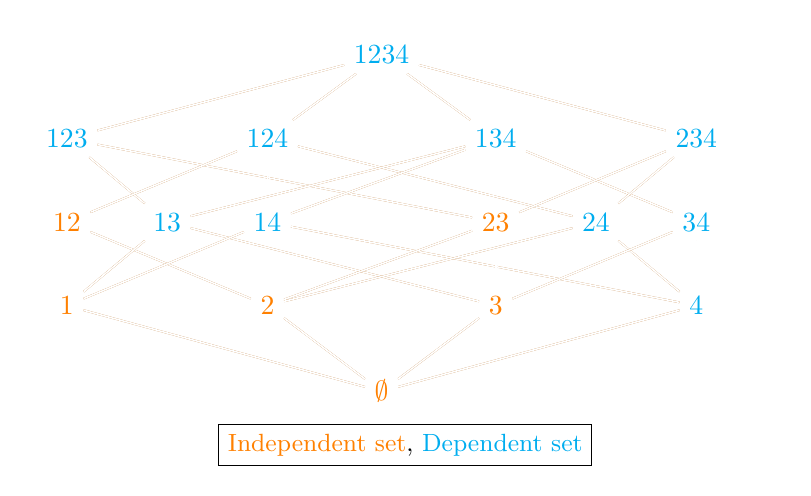
\begin{tikzpicture}

\matrix (a) [matrix of math nodes, column sep=0.6cm, row sep=0.6cm,]{
 & & &\textcolor{cyan}{
1234} & & & &\\
 \textcolor{cyan}{
123}& &\textcolor{cyan}{
124} & &\textcolor{cyan}{
134} &  & \textcolor{cyan}{
234}  \\
\textcolor{orange}{12} & \textcolor{cyan}{13} & \textcolor{cyan}{14} & & \textcolor{orange}{23} & \textcolor{cyan}{
24} & \textcolor{cyan}{
34} \\
\textcolor{orange}{1}& &\textcolor{orange}{2} & & \textcolor{orange}{3}& & \textcolor{cyan}{4} \\
& & & \textcolor{orange}{\emptyset} &  & & \\
&&&&&& \\};

\foreach \i/\j in {1-4/2-1, 1-4/2-3, 1-4/2-5, 1-4/2-7, 2-1/3-1, 2-1/3-2, 2-1/3-5, 2-3/3-1, 2-3/3-3, 2-3/3-6, 2-5/3-2, 2-5/3-3, 2-5/3-7, 2-7/3-5, 2-7/3-6, 2-7/3-7, 3-1/4-1, 3-1/4-3, 3-2/4-1, 3-2/4-5, 3-3/4-1, 3-3/4-7, 3-5/4-3, 3-5/4-5, 3-6/4-3, 3-6/4-7, 3-7/4-7, 3-7/4-5, 4-1/5-4, 4-3/5-4, 4-5/5-4, 4-7/5-4}
\draw[double, line width = 0.005mm, color = brown] (a-\i) -- (a-\j);

\node[draw] at (0, -2.5){\small \textcolor{orange}{Independent set}, \textcolor{cyan}{Dependent set}};

\end{tikzpicture} % why does it say this??? Did you forget a semicolon?
\end{center}
\caption{Diagram showing independent and dependent sets of a 4-element matroid.}
\end{figure}


The definition of a matroid is designed to extract out the property that makes a subset of elements 'independent'. This leads us to our first examples, namely the so-called \textit{representable matroids} arising from linear algebra. We would that a subset of vectors is \textit{independent} in a matroid, if and only if it is are \textit{linearly independent} in the usual sense. 
%This means, in particular, that the subsets have the same properties.



 Let $A \in \mat_{m \times n}(\mathbb{F})$ where $\mathbb{F}$ is a field. In the article we will not just be interested with $\mathbb{F} = \mathbb{C} \; \mathrm{or}\; \mathbb{F} = \mathbb{R} $ but also in finite fields 
 \footnote{In particular we are interested in $\mathbb{Z} / p\mathbb{Z}$ by which me mean integers modulo $p$ where $p$ is a prime number and will denote it by $\mathbb{F}_p$}.

\begin{exmp}
    

 
 We will pick a concrete example of $A \in  \mat_{3 \times 4}(\mathbb{R})$ to illustrate that the set of columns of a matrix has a natural matroid structure. Suppose

$$A = \begin{pmatrix}

2 & 0 & 2 & 0 \\
1 & -1 & 0 & 0 \\
0 & 3 & 3 & 0


\end{pmatrix}.$$

We would like to consider \textit{the set of labels of columns of the matrix $A$} and form a matroid on it. This means we start with $E = \{1,2,3,4\}$ so a finite set where the number $1$ corresponds to the column $\begin{pmatrix} 2 & 1 & 0 \end{pmatrix} ^ T$, the number 2 corresponds to $\begin{pmatrix}  0 & -1 & 3  \end{pmatrix} ^ T$ and so forth. We now declare that a subset of $E$ is called independent if and only if the corresponding set of column vectors is linearly independent as a set of vectors in $\mathbb{R}^3$. We can explicitly check what this means in our example. The sets $\{1\}$, $\{2\}$, $\{3\}$ are all independent because they correspond to non-zero vectors. For the two-element subsets we see that $\{1,2\}$, $\{1,3\}$ and $\{2,3\}$ are all independent, while any two element subsets containing the last column are not. Finally, the 3-element subset $\{1,2,3\}$ is not independent because as vectors, the first and the second column sum up to the third. So to conclude, the collection of all independent sets is
$$\mathcal{I} = \{\emptyset, \{1\}, \{2\}, \{3\}, \{1,2\}, \{1,3\}, \{2,3\} \},$$

which indeed satisfies the properties of collection of independent sets of a matroid. This is not a coincidence, we will prove that a collection of subsets formed from a matrix in the above way is always a matroid.

\end{exmp}


\begin{theorem}

    Let $A \in \mathrm{Mat} _{m \times n}(\mathbb{F})$ and $E = \{1, 2, \cdots, n\}$ be a finite set of $n$ elements where the element $i$ corresponds to the $i$-th column of the matrix $A$. We call a subset $I \subset E$ independent if and only if the column vectors that the members of $I$ correspond to form a linearly independent set as members of $\mathbb{F}^n$, and denote the collection of all independent subsets as $\mathcal{I}$. Then $M = (M, \mathcal{I})$ is a matroid, and we denote it by $M[A]$.
    
\end{theorem}

\begin{proof}
    We need to check that the collection $\mathcal{I}$ satisfies the three properties for the collection of independent sets given in the definition. 

\begin{enumerate}

    \item First, $\emptyset$ is trivially in $\mathcal{I}$.
    
    \item The second property is also satisfied because if $J \subset I$ and $I \in \mathcal{I}$ this means that the vectors corresponding to $I$ form a linearly independent set. In particular, let $v_1, v_2, \cdots v_j, v_{j+1}, \cdots v_{i}$ be the column vectors corresponding to $I$, and that first $j$ are also in $J$, that means $|I| = i$, $|J| = j$ and $j \leq i$. Then if for some linear combination we have $a_1v_1 + \cdots + a_jv_j = 0$, where $a_i \in \mathbb{F}$ then it is also true that $a_1v_1 + \cdots + a_jv_j + 0 \cdot a_{j+1} + \cdots + 0 \cdot a_i = 0$. Since the vectors of $I$ are linearly independent it now follows that $a_1 = a_2 = \cdots a_j = 0$ as well. So the vectors corresponding to the elements of $J$ are also linearly independent, which means by definition $J \in \mathcal{I}$.

    \item Finally, we have to check third property. We assume that $J, I \in \mathcal{I}$ and $|J| < |I|$. We denote by $V_J$ and $V_I$ the vector subspaces of $\mathbb{F}^n$ spanned by vectors corresponding to $J$ and $I$ respectively. Because the vectors corresponding to $J$ and $I$ respectively are linearly independent, they also form a basis for $V_J$ and $V_I$ respectively. For any $e \in I - J$ we denote by $v(e) \in \mathbb{F}^n$ the column vector of $A$ corresponding to $e$. Suppose some $e \in I - J$ has the property adding it to $J$ does not change the dimension of the subspace spanned by J, i.e. $\dim (V_J \cup v(e)) = \dim (V_J) = |J|$. Then $v(e)$ is already in $V(J)$ because the vectors corresponding to $J$ are linearly independent and if we do not increase the dimension, this means that $v(e)$ can be expressed as a linear combination of vectors corresponding to $J$. However, this cannot hold true for \textit{every} $e \in I - J$. If it would then for every $e \in I - J$, the vector $v(e) $ would already lie in $ V_J$, and because for all elements $i \in I \cap J$ we trivially have $v(i) \in V_J$ by definition, we would then have $V_I \subseteq V_J$. But this would mean that 

    $$|I| = \dim(V_I) = \dim(V_J) = |J| < |I|$$
     which is a contradiction. So there is at least one $e \in I - J$ so that $\dim(V_J \cup v(e)) = \dim(V_J) + 1$, which means the vectors corresponding to $J \cup e$ form a linearly independent subset. Finally, this means that $J \cup e \in \mathcal{I}$ which proves the third property.

\end{enumerate}
\end{proof}

In order to talk about any classification of matroids we have to say when the two matroids are equivalent - representing the same structure of independent sets. Intuitively, it is nothing deep, the definition will just rephrase that the two are \textit{equal} if it is possible to relabel the elements of the first matroid to the elements of the second without changing the independent sets.

\begin{defn}
    We call two matroids $M = (E, \mathcal{I})$ and $N = (F, \mathcal{J})$ isomorphic and denote it by $M \sim N$ if there exists a bijection $f: E \to F$ so that a subset $K \subset F$ is independent if and only if $K = f(L)$ for some independent set $L \in \mathcal{I}$.
\end{defn}


\begin{defn}
    We call a matroid $M$ representable, if $M$ is isomorphic to a matrix matroid $N[A]$ for some $A \in \mat_{m \times n}(\mathbb{F})$ over some field $\mathbb{F}$ and we call it $\mathbb{F}$-representable if it is representable over specific field $\mathbb{F}$.
\end{defn}

We will now define another important class of matroids. Due to its simplicity it will be suitable as an example in many of the notions defined in the proceeding text.

\begin{defn}
    Let $E = \{1, 2, \cdots, n\}$ and $\mathcal{I} = \{ L \subset E \; \text{ such that } \; |L| \leq m\}$. Then $(E, \mathcal{I})$ is a matroid which we denote by $U_{m,n}$ and call it a uniform matroid of rank $m$ on a $n$ element set.
\end{defn}
\begin{theorem}
    The ordered pair $U_{m,n} = (E, \mathcal{I})$ is a matroid
    
\end{theorem}

\begin{proof}
    
It is easy to check that $U_{m,n}$ is indeed a matroid. 


\begin{enumerate}
   

\item For any $m \geq 0$ we have $\emptyset \in \mathcal{I}$ since $|\emptyset | = 0$.

\item If $I \in \mathcal{I}$ and $J \subset I$ then $|J|\leq |I|$ so $|J|\leq |I| \leq m$ implying $J \in \mathcal{I}$ by definition.

\item  Finally, if $I, J \in \mathcal{I}$ and $|J|<|I|$ then for any $e \in I - J$ we will have $|J \cup e| = |J| + 1 \leq |I| \leq m$ so $J \cup e \in \mathcal{I}$ by definition for any $e \in I - J.$


\end{enumerate}
\end{proof}

\subsection{Bases}

Let $M = (E, \mathcal{I})$ be a matroid. We call a subset $B \subset E$ a \textit{basis} if it is a \textit{maximal independent set}. That means that $B$ is an independent set and $B$ is not properly contained inside any other independent set. It turns out that bases for matroids and bases in vector subspaces have some similarities in their properties. In particular the third property of independent sets immedietly guarantees us that all matroid bases have the same size, just like vector bases for finite-dimensional vector spaces.

\begin{theorem}
    Let $M = (E, \mathcal{I})$ be a matroid. All bases of $M$ have the same size.
\end{theorem}

\begin{proof}
    Suppose for contradiction that the theorem does not hold and, without loss of generality, let $B$ and $S$ be two bases with $|B| < |S|$ - different size. By the third property of independent sets we know there exists $e \in S - B$ such that $ B \cup e \in \mathcal{I}$. However, then $B$ is properly contained inside $B \cup e$, another independent set, which contradicts its maximality. So the initial assumption that there exist two bases with different size is false.
\end{proof}

The concept of a basis is important because it allows us to define a \textit{rank function} of a matroid which is the size of the maximal independent subset inside a given subset of a matroid.  Because the sizes of all of such sets - bases - are equal, this will be a well-defined notion.

Similar to the set of independent sets, we can characterize the set of bases of $M$ using these two properties:

\begin{defn}
    Let $E$ be a non-empty finite set, and $\mathcal{B}$ be a collection of subsets of $E$, called bases, with the following properties:
    \begin{enumerate}
        \item $\mathcal{B}$ is non-empty
        \item If $B_1,B_2\in\mathcal{B}$ and $x\in B_1 - B_2$, then there exists a $y\in B_2 - B_1$ such that $(B_1 - x)\cup y \in\mathcal{B}$.
    \end{enumerate}
    We will refer to these two properties as (B1) and (B2).
\end{defn}
Here below, you find a depiction of the matroid we have seen in chapter 2.1. This time, he have added the bases of the matroid, colored red. Two properties can be observed, first the bases are the maximal independent sets and both bases have two elements - the same size.

\begin{figure}[h]

\begin{center}
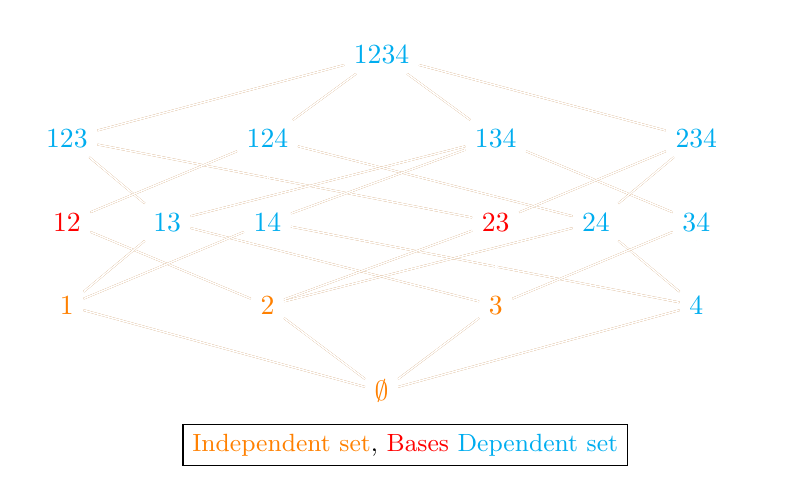
\begin{tikzpicture}

\matrix (a) [matrix of math nodes, column sep=0.6cm, row sep=0.6cm,]{
 & & &\textcolor{cyan}{
1234} & & & &\\
 \textcolor{cyan}{
123}& &\textcolor{cyan}{
124} & &\textcolor{cyan}{
134} &  & \textcolor{cyan}{
234}  \\
\textcolor{red}{12} & \textcolor{cyan}{13} & \textcolor{cyan}{14} & & \textcolor{red}{23} & \textcolor{cyan}{
24} & \textcolor{cyan}{
34} \\
\textcolor{orange}{1}& &\textcolor{orange}{2} & & \textcolor{orange}{3}& & \textcolor{cyan}{4} \\
& & & \textcolor{orange}{\emptyset} &  & & \\
&&&&&& \\};

\foreach \i/\j in {1-4/2-1, 1-4/2-3, 1-4/2-5, 1-4/2-7, 2-1/3-1, 2-1/3-2, 2-1/3-5, 2-3/3-1, 2-3/3-3, 2-3/3-6, 2-5/3-2, 2-5/3-3, 2-5/3-7, 2-7/3-5, 2-7/3-6, 2-7/3-7, 3-1/4-1, 3-1/4-3, 3-2/4-1, 3-2/4-5, 3-3/4-1, 3-3/4-7, 3-5/4-3, 3-5/4-5, 3-6/4-3, 3-6/4-7, 3-7/4-7, 3-7/4-5, 4-1/5-4, 4-3/5-4, 4-5/5-4, 4-7/5-4}
\draw[double, line width = 0.005mm, color = brown] (a-\i) -- (a-\j);

\node[draw] at (0, -2.5){\small \textcolor{orange}{Independent set}, \textcolor{red}{Bases} \textcolor{cyan}{Dependent set}};

\end{tikzpicture}
\end{center}
\caption{Diagram of a 4-element matroid}
\end{figure}

Let us prove that the set of bases of a matroid satisfy these conditions:
\begin{proof}
    To prove the first property observe that by defintion $\emptyset$ is always in $\mathcal{I}$ so the collection of independent sets is nonempty. This directly implies that the collection of bases is nonempty, for instance, an independent set with largest number of elements (there is at least one independent set! so we can talk about the largest one satisfying some properties) will be a basis, since it cannot be contained inside other independent set.
    
    
    For the second property let $x\in B_2 - B_1$. We first note that (I2) implies that $B_1 - x$ is independent, since it is a subset of $B_1$. Since $|B_1-x|<|B_2|$, we can apply (I3) on independent sets $B_1-x$ and $B_2$ to get that there exists a $y\in B_2-(B_1-x)$ such that $(B_1-x)\cup y \in\mathcal{I}$. Since $|(B_1-x)\cup y|=|B_1|$ and that all maximal independent sets have the same cardinality, $(B_1-x)\cup y$ must be a basis. Because $y$ is also in $B_2-B_1$, the property is fulfilled.    
\end{proof} 
Now that we have a new way to describe $\mathcal{B}$ with (B1) and (B2), we again need to prove that all elements in it are equicardinal. So let's do that.
\begin{proof}
    Suppose that $\mathcal{B}$ is not equicardinal, that is, we have $|B_1|<|B_2|$ for some $B_1,B_2\in\mathcal{B}$. From all $B_1,B_2$ where that holds, choose the pair that minimizes $|B_1-B_2|$. Since $B_1$ is bigger, choose an element $b\in B_1-B_2$ and apply (B2) to see that there exists a $d\in B_2-B_1$ such that $(B_1-b)\cup d \in\mathcal{B}$. With our choices of $b$ and $d$, we can see that $|((B_1-b)\cup d)-B_2|=|(B_1-b)-B_2|<|B_1-B_2|$. This, combined with that $|(B_1-b)\cup d|=|B_1|<|B_2|$, tells us that $B_1$ and $B_2$ are actually not the minimal choice. This contradiction proves that $\mathcal{B}$ is equicardinal.
\end{proof}

To prove that the two properties are sufficient to describe the bases of $M$, we will that if $\mathcal{B}$ is any collection of subsets satisfying the bases axioms, then the independent sets should be all of the possible subsets of the the elements of $\mathcal{B}$:
\begin{theorem}
    Let $\mathcal{B}$ be a collection of subsets of a non-empty finite set $E$, satisfying (B1) and (B2). Let $\mathcal{I}=\{ I\subset B : B\in\mathcal{B} \}$. Then $(E,\mathcal{I})$ is a matroid with $\mathcal{B}$ as its set of bases.
\end{theorem}
\begin{proof}
    Our goal is of course to show that $\mathcal{I}$ satisfies the conditions of independent sets. If we manage to do that we will have that $(E, \mathcal{I})$ is a matroid having $\mathcal{B}$ as its collection of bases.
    \begin{enumerate}
        \item Since (B1) tells us that $\mathcal{B}$ is nonempty and because $\emptyset$ is a subset of any set, in particular $\emptyset \subset B$ where $B$ is some member of $\mathcal{B}$, we by definition have that $\emptyset \in \mathcal{I}$.
        
        \item If $I\in\mathcal{I}$ and $J\subset I$, then by construction, $J\subset I\subset B$ for some $B\in\mathcal{B}$, which means that $J\in\mathcal{I}$. So $\mathcal{I}$ satisfies (I2).
        
        \item Suppose (I3) fails for some $I,J\in\mathcal{I}$ with $|I|<|J|$. That means for all elements $x\in J-I$, $I\cup x \notin \mathcal{I}$. Let $B_I$ and $B_J$ be the elements of $\mathcal{B}$ that contain $I$ and $J$, respectively, and choose the $B_J$ so that $|B_J - (J\cup B_I)|$ is minimal. 
    
        With our choice of $I$ and $J$, it turns out that $J-B_I = J-I$. If this would not be the case, then there would be an element $e$ in $B_I-I$ that is also in $J$. However, then $I\cup e\notin \mathcal{I}$, which contradicts $I\cup e\subset B_I$.

        Suppose now that $B_J-(J\cup B_I)$ is non-empty. Letting $j$ be an element from this set, (B2) tells us that there is an element $i\in B_I-B_J$ such that $(B_J-j)\cup i \in\mathcal{B}$. However, then $|((B_J-j)\cup i)-(J\cup B_I)|=|(B_J-j)-(J\cup B_I)|<|(B_J-(J\cup B_I)|$, which contradicts the minimality of our choice of $B_J$. Thus, $B_J-(J\cup B_I)=\emptyset$. This now implies that $B_J\subset J\cup B_I$, which implies that $B_J-B_I\subset (J\cup B_I)-B_I=J-B_I$. Since $J-B_I\subset B_J-B_I$, this proves equality between $B_J-B_I$ and $J-B_I$.

        Next up we do the same thing, but this time proving that $B_I-(I\cup B_J$ is empty. Assuming the opposite by letting $i$ be a part the set, (B2) tells us that there exists a $j\in B_J-B_I=J-B_I=J-I$ such that $(B_I-i)\cup j\in\mathcal{B}$. Since our choice of $i$ tell us that $I\cup j\subset (B_I-i)\cup j$, it means $I\cup j\in\mathcal{I}$. This gives us precicely (I3), which contradicts our originil assumption. Thus, $B_I-(I\cup B_J)=\emptyset$. By the same logic we used in the previous paragraph, $B_I-B_J=I-B_J\subset I-J$.

        We can use the fact that $\mathcal{B}$ is equicardinal to see that $|B_I-B_J|=|B_J-B_I|$. At last, we use all of our knowledge to get the following:
        $$ |I-J|\geq |B_I-B_J|=|B_J-B_I|=|J-B_I|=|J-I| $$
        This inequality tells us that $|I|\geq |J|$, which is a contradiction with another one of our assumptions. Thus, $\mathcal{I}$ satisfies (I3). And thus, $(E,\mathcal{I})$ is a matroid.
    \end{enumerate}  
    The fact that $\mathcal{B}$ is now the set of bases of the matroid $(E,\mathcal{I})$ follows from the fact that all elements in $\mathcal{B}$ are maximal in $\mathcal{I}$.
\end{proof}



\newpage

\subsection{Circuits} 
As mentioned before we can define a matroid in different forms, one of this other definitions is in terms of circuits. Before the definition, we need to introduce an additional concept. 
That is, a minimal dependent set, these are dependent sets whose all proper subsets are independent.

Now, we can state the following:
\begin{defn}
Let $M = (E, \mathcal{I})$ be a matroid. Any subset $D \in \mathcal{I}$ which is not independent is called dependent. Circuit will be a minimal dependent set of an arbitrary matroid $M$. The collection will be denoted by $C$ or $\mathcal{C}(M)$. Additionally, we define a circuit of a matroid $M$, that has $n$ elements, as an $n$-circuit.
\end{defn}

The name is a reference to matroid circuits corresponding to circuits of the underlying graph when talking about graphic matroids.

Similarly, as with the independent sets, we can use the circuits to formulate a definition for a given matroid. And moreover, in the same way we can use the independent sets of a matroid to determine its circuits, we can use the circuits of a matroid to determine its independent sets.

So, we can characterize the concept of a matroid in the following way:

\begin{defn}
    Let $E$ be a non-empty finite set, and $\mathcal{C}$ a collection of subsets of $E$, called circuits, such that:

    \begin{enumerate}
        \item $\emptyset \notin \mathcal{C}$

        \item If $C_1$ and $C_2$ are members of $\mathcal{C}$ and $C_1 \subseteq C_2$, then $C_1 = C_2$.

        \item If $C_1$ and $C_2$ are distinct members of $\mathcal{C}$ and there exist an $e \in C_1 \cap C_2$, then there is a member $C_3$ of $\mathcal{C}$, such that $C_3 \subseteq (C_1  \cup C_2) - e$
    \end{enumerate}
    We will refer to these three properties as (C1), (C2) and (C3)
    
\end{defn}

Again, we will use the same matroid example as before, this time adding circuits to the drawing (in blue). As you can see, the circuits are minimal dependent sets where everything above it is a dependent set. Also note how all independent sets do not contain any circuit.

\begin{center}
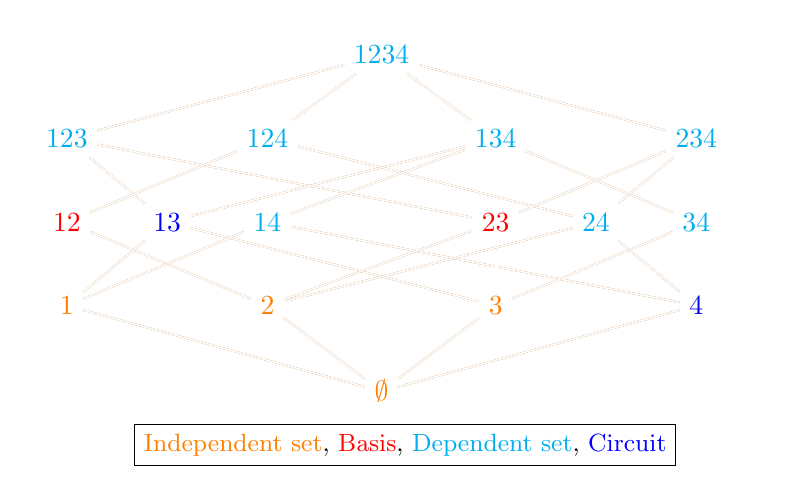
\begin{tikzpicture}

\matrix (a) [matrix of math nodes, column sep=0.6cm, row sep=0.6cm,]{
 & & &\textcolor{cyan}{
1234} & & & &\\
 \textcolor{cyan}{
123}& &\textcolor{cyan}{
124} & &\textcolor{cyan}{
134} &  & \textcolor{cyan}{
234}  \\
\textcolor{red}{12} & \textcolor{blue}{13} & \textcolor{cyan}{14} & & \textcolor{red}{23} & \textcolor{cyan}{
24} & \textcolor{cyan}{
34} \\
\textcolor{orange}{1}& &\textcolor{orange}{2} & & \textcolor{orange}{3}& & \textcolor{blue}{4} \\
& & & \textcolor{orange}{\emptyset} &  & & \\
&&&&&& \\};

\foreach \i/\j in {1-4/2-1, 1-4/2-3, 1-4/2-5, 1-4/2-7, 2-1/3-1, 2-1/3-2, 2-1/3-5, 2-3/3-1, 2-3/3-3, 2-3/3-6, 2-5/3-2, 2-5/3-3, 2-5/3-7, 2-7/3-5, 2-7/3-6, 2-7/3-7, 3-1/4-1, 3-1/4-3, 3-2/4-1, 3-2/4-5, 3-3/4-1, 3-3/4-7, 3-5/4-3, 3-5/4-5, 3-6/4-3, 3-6/4-7, 3-7/4-7, 3-7/4-5, 4-1/5-4, 4-3/5-4, 4-5/5-4, 4-7/5-4}
\draw[double, line width = 0.005mm, color = brown] (a-\i) -- (a-\j);

\node[draw] at (0, -2.5){\small \textcolor{orange}{Independent set}, \textcolor{red}{Basis}, \textcolor{cyan}{Dependent set}, \textcolor{blue}{Circuit}};

\end{tikzpicture}
\end{center}

To get an intuition behind (C3), let us consider the matroid induced by the graph above. We will discuss graphic matroid later, but just know that a circuit is a cycle in the graph. Here, we have two circuits, $C_1$ and $C_2$, that share an edge, $e$. If you take the union of both circuits and remove the edge $e$ from it, then that subgraph contains another cycle, circuit $C_3$.

% Someone please fix this!


\begin{figure}
\caption{A graph of suspicious shape, having three cycles.}
\begin{subfigure}[h]{0.245\textwidth}
  \caption{Graph}
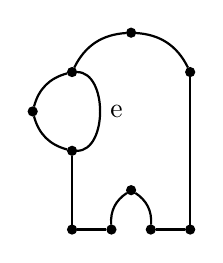
\begin{tikzpicture}[node distance={10mm}, thick, main/.style = {draw,circle,fill,inner sep=1pt}] 
  \node[main] (1) at (0,0) {}; 
  \node[main] (3) at (-0.5,0.5) {}; 
  \node[main] (4) at (0, 1) {}; 
  \node[main] (5) at (0, -1) {}; 
  \node[main] (6) at (1.5, -1) {}; 
  \node[main] (7) at (0.75, 1.5) {}; 
  \node[main] (8) at (1.5, 1) {}; 
  \node[main] (9) at (0.5, -1) {}; 
  \node[main] (10) at (1, -1) {}; 
  \node[main] (11) at (0.75, -0.5) {}; 
  \draw (1) to [bend left] (3);
  \draw (1) to [bend right=90]
node[midway, right] {e} (4) ;
  \draw (3) to [bend left] (4);
  \draw (4) to [bend left] (7);
  \draw (7) to [bend left] (8);
  \draw (8) to (6);
  \draw (5) to (9);
  \draw (6) to (10);
  \draw (9) to [bend left] (11);
  \draw (10) to [bend right] (11);
  \draw (5) to (1);
\end{tikzpicture} 
\end{subfigure}
\begin{subfigure}[h]{0.245\textwidth}
  \caption{$C _1$}
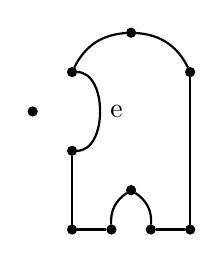
\begin{tikzpicture}[node distance={10mm}, thick, main/.style = {draw,circle,fill,inner sep=1pt}] 
  \node[main] (1) at (0,0) {}; 
  \node[main] (3) at (-0.5,0.5) {}; 
  \node[main] (4) at (0, 1) {}; 
  \node[main] (5) at (0, -1) {}; 
  \node[main] (6) at (1.5, -1) {}; 
  \node[main] (7) at (0.75, 1.5) {}; 
  \node[main] (8) at (1.5, 1) {}; 
  \node[main] (9) at (0.5, -1) {}; 
  \node[main] (10) at (1, -1) {}; 
  \node[main] (11) at (0.75, -0.5) {}; 
  \draw (1) to [bend right=90]
node[midway, right] {e} (4) ;
  \draw (4) to [bend left] (7);
  \draw (7) to [bend left] (8);
  \draw (8) to (6);
  \draw (5) to (9);
  \draw (6) to (10);
  \draw (9) to [bend left] (11);
  \draw (10) to [bend right] (11);
  \draw (5) to (1);
\end{tikzpicture} 
\end{subfigure}
\begin{subfigure}[h]{0.245\textwidth}
  \caption{$C _2$}
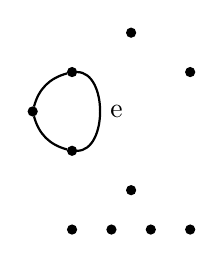
\begin{tikzpicture}[node distance={10mm}, thick, main/.style = {draw,circle,fill,inner sep=1pt}] 
  \node[main] (1) at (0,0) {}; 
  \node[main] (3) at (-0.5,0.5) {}; 
  \node[main] (4) at (0, 1) {}; 
  \node[main] (5) at (0, -1) {}; 
  \node[main] (6) at (1.5, -1) {}; 
  \node[main] (7) at (0.75, 1.5) {}; 
  \node[main] (8) at (1.5, 1) {}; 
  \node[main] (9) at (0.5, -1) {}; 
  \node[main] (10) at (1, -1) {}; 
  \node[main] (11) at (0.75, -0.5) {}; 
  \draw (1) to [bend left] (3);
  \draw (1) to [bend right=90]
node[midway, right] {e} (4) ;
  \draw (3) to [bend left] (4);
\end{tikzpicture} 
\end{subfigure}
\begin{subfigure}[h]{0.245\textwidth}
  \caption{$C _3$} 
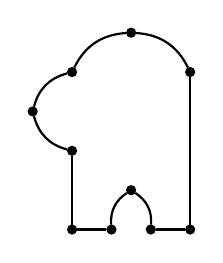
\begin{tikzpicture}[node distance={10mm}, thick, main/.style = {draw,circle,fill,inner sep=1pt}] 
  \node[main] (1) at (0,0) {}; 
  \node[main] (3) at (-0.5,0.5) {}; 
  \node[main] (4) at (0, 1) {}; 
  \node[main] (5) at (0, -1) {}; 
  \node[main] (6) at (1.5, -1) {}; 
  \node[main] (7) at (0.75, 1.5) {}; 
  \node[main] (8) at (1.5, 1) {}; 
  \node[main] (9) at (0.5, -1) {}; 
  \node[main] (10) at (1, -1) {}; 
  \node[main] (11) at (0.75, -0.5) {}; 
  \draw (1) to [bend left] (3);
  \draw (3) to [bend left] (4);
  \draw (4) to [bend left] (7);
  \draw (7) to [bend left] (8);
  \draw (8) to (6);
  \draw (5) to (9);
  \draw (6) to (10);
  \draw (9) to [bend left] (11);
  \draw (10) to [bend right] (11);
  \draw (5) to (1);
\end{tikzpicture} 
\end{subfigure}
                  \end{figure}

We can say that a set $X \subseteq E$ is independent if and only if, it does not contain any circuit.

The concept of circuits points towards the direction of something similar to a complement of the independent sets, but not completely, since it is only the minimal dependent, and not all dependet subsets. We now have the following theorem.

\begin{lemma}\label{lem:circuits-have-properties}
  All circuits in a matroid satisfy (C1), (C2) and (C3).
\end{lemma}

\begin{proof} We will prove each property individually:
  
\begin{enumerate}
    \item $\emptyset \in \mathcal I$, therefore $\emptyset$ is not dependent (which means it cannot be a circuit)
    \item A counterexample to this clause would violate the $C _2$ being minimal.
    \item Assume a counterexample exists. Because $C _1 \cup C _2 - e$ does not contain a circuit, it must be an element of $\mathcal I$. 

        We claim that $C _2 \setminus C _1$ is nonempty. Assume this is not the case. That would imply $C _2 \subseteq C _1$, but $C _1 \neq C _2 $ by (C3), which means that $C _1 $ is a proper subset of $C _2$. As both $C _1 $ and $C _2 $ are members of $\mathcal C$, this violates (C2), and is a contradiction. We can then assume some $f \in C _2 \setminus C _1 $ exists.

        As $C _2$ is minimally dependent, we know that $C _2 - f$ is independent. Let $I$ be a maximal independent subset of $C _2 \cup C _1$ which is a superset of $C _2 - f$. Clearly, $f \not\in I$ (otherwise $C _2 \subseteq I \in \mathcal I$). Furthermore, as $C _1 $ is a circuit, we know that $C _1 \not \subseteq I \in \mathcal I$ (otherwise $C _1$ would be independent). This means some $g \in C _1$ exists such that $g \not\in I$. As $f \in C _2  \setminus  C _2$, we know that $f \neq g$.

        As $I \subseteq C _1 \cup C _2$ and $f, g \in C _1 \cup C _2$ but $f, g \not\in I$, we can infer that 
        \begin{align*}
        |I| \leq |C _1 \cup C _2 - f - g| = |C _1 \cup C _2| - 2.
        \end{align*}

        We also notice that $|C _1 \cup C _2 - e| = |C _1 \cup C _2 | - 1$. We can now conclude by transitivity with $|C _1 \cup C _2 | - 2 < |C _1 \cup C _2 | - 1$ that $|I| < |C _1 \cup C _2 - e|$. We recall that both $I$ and $C _1 \cup C _2 - e$ are members of $\mathcal I$. We can apply (I3) to generate a superset of $I$ which contradicts it's maximallity.
\end{enumerate}
\end{proof}

\begin{theorem}\label{thm:matroid-circuit-definition}
Let $E$ be a set and $\mathcal C$ be a collection of subsets of $E$ which satisfies the conditions outlined above. Let  $\mathcal I$  be the collection of subsets of $E$ that contain no member of $\mathcal C$, that is 

\begin{align}
   % \forall X \in \mathcal{I}, \forall C \in \mathcal C,  C \not \subseteq X. 
   \mathcal{I} = \{I \in 2^E |\; \text{for all } \; C \in \mathcal{C}\; \text{we have} \; C \not\subset I\}
    \label{independent-sets-from-circuits}
\end{align}

    The pair $(E,\mathcal I)$ is a matroid having $\mathcal C$ as its collection of circuits.
\end{theorem}

\begin{proof} We start by showing that $\mathcal I $ satisfies the necessary conditions for $(E, \mathcal I )$ to be a matroid:
    \begin{enumerate} 
        \item The only subset of $\emptyset $ is $ \emptyset $, but $ \emptyset \not\in \mathcal C $, so $ \emptyset $ satisfies (\ref{independent-sets-from-circuits}), hence $\emptyset \in \mathcal I$.
    \item Assume we have $X \subseteq Y \in \mathcal I$. Assume that $X \not\in I$, i.e.\ there exists some $C \in \mathcal C $ such that $C \subseteq X$. We recall that $\subseteq $ is transitive, thus $C \subseteq Y$ and $Y \not\in I$, hence a contradiction.
    \item Given $X, Y \in \mathcal I $ with $|X| < |Y|$ we must show there exists some $e \in Y \setminus X$ such that $X \cup \{e\} \in \mathcal I$. Assume that such an $e$ does not exist, i.e.\ for all $e \in Y \setminus X$ we have some circuit $C _e \in \mathcal C $ such that $C _e \subseteq X \cup \{e\}$. We obviously have $e \in C_e$, because otherwise $C_e \subseteq X$ and $X \not\in \mathcal I$.


     Let $X' = X \setminus Y$ and $Y' = Y \setminus X$. We will prove the statement by induction: given some set $S \subseteq X'$, a set of circuits $D \subseteq \mathcal C$ with $\forall C \in D, C \subseteq  S \cup Y$ and a surjective but not injective function $f : D \to S$ such that $f(D)$ is maximal in size and $\forall C \in D, f(C) \in C$, our statement is proven. We will use induction on the size of $S$:
    \begin{enumerate}
      \item If $S = \{e\}$ only has one element, we know that $f$ is not injective, so we must have distinct $C _1, C _2 \in D$ such that $e = f(C _1 ) = f(C _2)$. We can use the $3$-rd circuit axiom to generate some circuit $C _3 \subseteq C _1 \cup C _2 - e$. We recall that $C _1 , C _2 \subseteq S \cup Y $, so $C _3 \subseteq S \cup Y - e$ which implies $C _3 \subseteq Y$, which is a contradiction.
        \item Inductive step. Assuming the statement is true for all choices of $S$ with $k$ elements, we will attempt to prove it is also true when $S$ has $k + 1$ elements. Recalling that $f$ is not injective, we must have distinct $C _1, C _2 \in D$ such that $f(C _1 ) = f(C _2)$. Let $g = f(C _1)$. We have $g \in C _1, C _2$, so by the $3$-rd circuit axiom we must have some circuit $C  _3 \subseteq C _1 \cup C _2 - g$. Let $S' = C _3 \cap X'$. 

            For all $e \in S'$, we claim there must exist some $C_e \in D$ such that $e = f(C_e)$. Assume this is not the case, i.e.\ there is some $e \in S'$ such that no valid choice of $C_e$ exists. Given that $e \in S'$, we know that either $e \in C_1$ or $e \in C_2$. After a potential swap, we assume that $e \in C_1$. We can now define $f'(C) = e$ when $C = C_1$ and $f'(C) = f(C)$. Because no choice of $C_e$ exists, we know that $e \not\in f(D)$. Because $f(C _1 ) = f(C _2 )$ we have $f(D) = f(D - C _1 )$ which lets us compute $f'(D) = f(D) \cup \{e\}$, which means $f(D)$ was not maximal, hence a contradiction. Our claim is then true.

            Define $D' = \{C_e | e \in S'\} \cup \{C _3 \}$. We've essentially proven in the last paragraph that $f : \{C_e | e \in S'\} \to S'$ is still a  surjective function. It then follows that $h = f : D' \to S'$ is surjective as well. By the Pigeonhole principle, we know $h$ cannot be injective, because $|D'| = |S'| + 1$. We are now almost ready to apply the induction hypothesis to $(S', D', h)$. We've shown a choice for $h$ exist. If this choice is not maximal, swap it with a maximal choice (we had to show that at least one choice exists for a maximal choice to exist). We can now apply the induction hypothesis, proving the statement.
    \end{enumerate}

    We notice that $X$ can be partitioned into $X'$ and $X \cap Y$, hence $|X| = |X'| + |X \cap Y|$. We can follow a similar process for $Y$. Combining the two together with the fact that $|X| < |Y|$ yields that $|X'| < |Y'|$. We know that $Y \in \mathcal I$ so $\forall e \in Y', C_e \not \subseteq  Y$, but $C_e \subseteq  X \cup \{e\}$ therefore there must exist some $c_e \in C_e \cap X'$. 

    We define $D = \{C_e, e \in Y'\}$, $f(C_e) = c_e$ and $S = f(D)$. Furthermore, we know that $f$ is not injective by the Pigeonhole principe (we have $|D| = |Y'| > |X'| \geq |S|$). We also know, by the definition of $S$, that $f$ is surjective. We've shown a choice of $f$ exists. If it is not maximal, swap it with a maximal choice. We can now apply the statement proven by induction to finish the proof.
\end{enumerate}


We now show that $C$ is a circuit for the newly defined matroid if and only if it is a member of $\mathcal C$. 
\begin{enumerate}
  \item[$\implies$]
  If $C$ is a circuit, then $C \not\in \mathcal I$, which means that $C$ contains some $D \in \mathcal C$. As $C$ is minimally dependent, all it's proper subsets are independent, but members of $\mathcal C$ cannot be independent (as seen in the definition of $\mathcal I$), which implies that $C = D$, hence $C \in \mathcal C$.
  \item[$\impliedby$]
  Let $C \in \mathcal C$. Assume $C$ is not a circuit. Clearly, $C \not\in \mathcal I$ is implied by the definition of $\mathcal I$ seen above. This implies that $C$ is dependent but not a circuit, which means $C$ is not miminal. 

  A proper subset $D  \subsetneq C$ must then exist such that $D$ is a circuit. We've already shown in the $\implies$ direction how this implies $D \in \mathcal C$. We have now constructed a contradiction to (C2), hence our assumption that such a circuit exists is false.

\end{enumerate}



  We can now conclude that $(E, \mathcal I)$ is indeed a matroid with $\mathcal C$ as it's set of circuits.
\end{proof}

\section{Graphic matroids}

TRYING TO DO GRAPHS, DONT LAUGH! (DO NOT TOUCH!)

First, we do not define graphs in completely the same way as in the graph theory class. We used the definition that a graph $G$ is an ordered pair $G = (V, E)$ where $V$ is a finite set (of vertices) and $E$ is a collection of two-element subsets of $V$ (of edges). We will extend the notion of edge to include \textit{loops} and \textit{parallel edges}. For this, we will first illustrate the two notions. Intuitively a loop is an edge going from a vertex to itself, one can also have multiple loops on a single vertex.


For example, in the figure \ref{ilustratinloops}, we have a vertex $a$ with a single loop and vertex $d$ with 3 loops.

\begin{figure}[H]
    \centering
    \subfloat[\centering Loops]{
    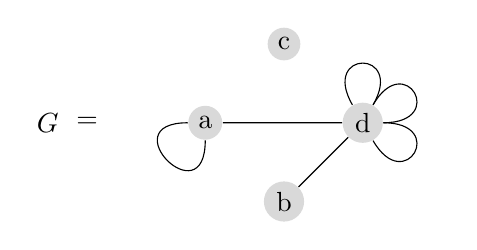
\begin{tikzpicture}[every loop/.style={}]

  \tikzstyle{vertex}=[circle,fill=black!15,minimum size=8pt,inner sep=2pt]

  \node (name) at (-2,0) {$G $};
  \node (another name) at (-1.5,0) {$ =$};
   
  
  \node[vertex] (v2) at (0,0)   {a};
  \node[vertex] (v3) at (1,-1)  {b};
  \node[vertex] (v4) at (1,1)  {c};
  \node[vertex] (v5) at (2,0)  {d};
  \draw (v2) edge[in=270,out=180, loop] node[below] {} ();

  \draw (v5) edge[in=300,out=0, loop] node[below] {} ();
  \draw (v5) edge[in=0,out=60, loop] node[below] {} ();
  \draw (v5) edge[in=60,out=120, loop] node[below] {} ();

  \draw (v2) -- (v5) -- (v3) -- cycle;

  
  %\draw[step=1cm,gray,very thin] (-2,-2) grid (4,4);

%\draw (v1) edge[in=270,out=180, loop] node[below] {2} ();

 
  
\end{tikzpicture}
    
    
    }%
    \qquad
    \subfloat[\centering Parallel edges]{
    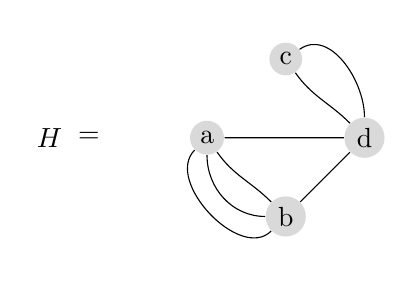
\begin{tikzpicture}[every loop/.style={}]

  \tikzstyle{vertex}=[circle,fill=black!15,minimum size=8pt,inner sep=2pt]

  \node (name) at (-2,0) {$H $};
  \node (another name) at (-1.5,0) {$ =$};
   
  
  \node[vertex] (v2) at (0,0)   {a};
  \node[vertex] (v3) at (1,-1)  {b};
  \node[vertex] (v4) at (1,1)  {c};
  \node[vertex] (v5) at (2,0)  {d};
  
  \draw (v2) edge[in=225,out=225] node[below] {} (v3);
  \draw (v2) edge[in=180,out=270] node[below] {} (v3);
  \draw (v2) edge[in=135,out=305] node[below] {} (v3);

  \draw (v4) edge[in=135,out=305] node[below] {} (v5);
  \draw (v4) edge[in=90,out=35] node[below] {} (v5);


  \draw (v2) -- (v5) -- (v3) -- cycle;

  
  %\draw[step=1cm,gray,very thin] (-2,-2) grid (4,4);

%\draw (v1) edge[in=270,out=180, loop] node[below] {2} ();

 
  
\end{tikzpicture}
    }%
    \caption{Graph $G$ with loops and graph $H$ with parallel edges}%
    \label{ilustratinloops}%
\end{figure}


Above we see graphs $G$ and $H$, one has loops and the other has parallel edges. One way to formalize both constructions, as done in \cite{oxley1} (for them to behave in the way we would like them to behave) is to define a graph to be an ordered pair $(V, E)$, where $V$ is a finite set, so unchanged, however $E$ is a \textit{multiset} of edges. This allows the same two-element subset of $V$ to appear multiple (but at most finitely many) times in $E$, even though it is the same set. Hence, we get parallel edges. For loops, we can get to a multiset consisting of a single element twice, and we also allow it to appear multiple times...
However, the formal construction is not so important, as we will see in the future and one can usually restrict to simple graphs, which are by our terminology the ones without loops or parallel edges. However, we are interested in \textit{properties} loops and parallel edges have. In particular, we see that by our definition of a cycle (a path (a walk (a sequence of adjacent vertices) which does not repeat vertices) which can repeat only one vertex (the ending and the starting vertex)), we have that if a loop is in a cycle, then the whole cycle consists only of that loop - we have one vertex appearing multiple times in a sequence - the beginning/ending vertex. Also, for parallel edges, at most one from a class of parallel edges connecting the same two vertices can appear in a cycle.


\begin{figure}[H]
\centering

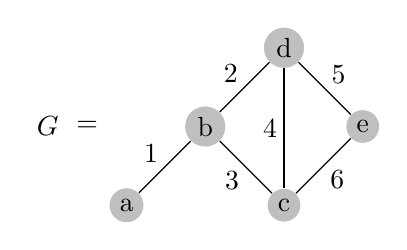
\begin{tikzpicture}[every loop/.style={}]

      \tikzstyle{vertex}=[circle,fill=black!25,minimum size=6pt,inner sep=2pt]

  \node (name) at (-2,0) {$G $};
  \node (another name) at (-1.5,0) {$ =$};
   
  \node[vertex] (v1) at (-1,-1) {a};
  \node[vertex] (v2) at (0,0)   {b};
  \node[vertex] (v3) at (1,-1)  {c};
  \node[vertex] (v4) at (1,1)  {d};
  \node[vertex] (v5) at (2,0)  {e};
  \draw (v1) -- node[midway, xshift=-0.5em, yshift=0.5em]{1} (v2) -- node[midway, xshift=-0.5em, yshift=-0.5em]{3} (v3) -- cycle;
  \draw (v2) -- node[midway, xshift=-0.5em, yshift=0.5em]{2} (v4) -- node[midway, xshift=0.5em, yshift=0.5em]{5} (v5) -- node[midway, xshift=0.5em, yshift=-0.5em]{6} (v3) -- cycle;
  \draw (v4) -- node[midway, xshift=-0.5em, yshift=0em]{4} (v3);

  
  %\draw[step=1cm,gray,very thin] (-2,-2) grid (4,4);

%\draw (v1) edge[in=270,out=180, loop] node[below] {2} ();

 
  
\end{tikzpicture}
\caption{Simple graph on 6 edges}
  \label{simp}

\end{figure}

Consider a concrete example of a simple graph and build a matroid out of it. Let us label the set of edges $E = \{1, 2, 3, \cdots, 6\}$. We will define a collection of subsets $\mathcal{C}$ of $E$ where $C \in \mathcal{C}$ if and only if the set of edges of $C$ forms a cycle in $G$. We check that 

    $$\mathcal{C} = \{\{2,3,4\}, \{4,5,6\}, \{2, 3, 5, 6\}\}.$$

Not surprisingly, the set $E$ with the collection $\mathcal{C}$ being as its set of circuits is, in fact, a matroid, we can check that there is no $\emptyset$ in $\mathcal{C}$, none of its members is properly contained in each other, and finally "circuit elimination axiom" works for all three possibilities of taking pairs of elements of $\mathcal{C}$. We will now prove that this works for a general graph.

\begin{theorem}
Let $G = (V, E)$ be a graph and let $C_1$, $C_2$ be sets of edges of two distinct cycles with a nonempty intersection. Then for any $e \in C_1 \cap C_2$ there exists a cycle $C_3 \subset C_1 \cup C_2 -e$, making the set $E$ of edges into a matroid with the set of circuits equal to the collection of cycles.
\end{theorem}

\begin{proof}

Let the cycle $C_1$ correspond to the sequence of incident vertices  $v_0, \cdots, v_n = v_0$ and let without loss of generality the special edge in the interesection be the edge $e = \{v_0, v_1\}$. Our goal is to find a cycle in the set of edges $C_1 \cup C_2 -e$, which is not difficult, the idea is that we go around $C_1$ until we can jump to $C_2$ for the first time, then we go back to $e$ via $C_2$ from the "backward direction".

Let $k$ be the smallest integer $1<k\leq n$ such that the vertex $v_k$ is in the cycle $C_2$. We know that such an integer exists because $v_n$ is in the cycle $C_2$. 

Let $v_k, w_{k+1}, w_{k+2}, \cdots, v_1$ be the path of vertices in the cycle $C_2$ which does not include the edge $e$. We know that such a path exists, because $C_2$ is a cycle, so from any two distinct vertices, in particular $v_k$ and $v_1$ there are two paths going from $v_k$ to $v_1$ including only the vertices of $C_2$ - we pick the one that does not include the edge $e$.

We claim that the cycle consisting of vertices $v_1, v_2, \cdots v_k, w_{k+1}, \cdots , v_1$ is the desired one and denote its set of edges by $C_3$. By construction the sequence of vertices $v_1, v_2, \cdots v_k, w_{k+1}, \cdots , v_1$ is a cycle, namely the neighboring vertices are incident and except $v_1$ there is no vertex repeating, because we have chosen $v_2, v_3, \cdots v_{k-1}$ to be disjoint from $C_2$. Crucially, $e \notin C_3$ because we have chosen path $v_k, w_{k+1}, \cdots v_1$ to not include the edge $e$ and $v_1, v_2, \cdots v_k$ does not include it because $e = \{v_n = v_0, v_1\}$ and there is no $v_0$ in our cycle. Finally, all of the vertices of $C_3$ are inside the vertices of $C_1$ and $C_2$ by construction so, to conclude the set $C_3$ has the desired property $C_3 \subset (C_1 \cup C_2) - e$.

We have to check to check the possibility that $e$ might be a loop or a parallel edge as well, the above argument works assuming $G$ is a simple graph. If $e$ is a parallel edge than the above argument does still hold since we only now that there is more than one edge between $v_0$
and $v_1$ which does not change anything. However, if $e$ is a loop then by our convention, a cycle consisting of a loop can just be that loop and nothing else, heuristically, because it begins and ends at a single vertex. So $C_1 = C_2 = \{e\}$ which is a contradiction, since we have assumed $C_1$ and $C_2$ are distinct.

To show that the set $E$ is a matroid with the collection $\mathcal{C}$ of cycles as circuits we only have to verify the first two circuit axioms. The empty set is by our defintion not a cycle, because by our defintion a cycle always includes a nonempty set of vertices it is build upon. If there are at least two vertices, than we have incident edges inside, and the only cycle on one vertex is a loop, which is still an edge.

The show the first property suppose we have two sets of edges of cycles such that $C_1 \subset C_2$ and assume for contradiction there is some $e \in C_2 - C_1$. Then (we are assuming neither of the cycles are loops, that case is obvious) the set of edges $C_2 - e$ corresponds to a path from the vertices which $e$ connects. However there is a cycle $C_1 \subset C_2 -e$ which is a subset of a path - a contradiction. So if $C_1 \subset C_2$ then $C_2 - C_1$ is empty, in particular then $C_2 = C1$ and all three circuit axioms are satisfied.



\end{proof}

\begin{defn}
    We call a matroid $M$ graphic it is isomporphic to $(E, \mathcal{I})$ where $E$ is the set of edges of some graph and the set of circuits is given by the set of all edge cycles.
\end{defn}

We thus know that given any graph $G$ we have natural matroid structure on its set of edges, by declaring graph cycles to be circuits. Because we know other equivalent descriptions of matroids it is natural to ask what are the independent sets or bases in the case of graphic matroids. 

Suppose that the set of edges $B$ is a base of a graphic matroid. We know that this means that $B$ is independent (interpretation of which in the case of graphic matroids we do not yet know) however, adding any element of $E-B$ to $B$, i.e. any edge not in $B$ to $B$, we get a \textit{dependent set}, which means it contains a circuit. By our defintion this means that it has to contain an edge cycle. Combining all we see that the set of edges $B$ has the property that it does not contain any cycles, however adding any edge makes a cycle - this is the precisely one of the equivalent characterizations of \textit{spanning forrests} - we cannot say spanning trees because the graph might not be connencted. 

Any independent set is a subset of some basis, so in graphic matroids the set of edges that is independent has to be a subset of some spanning forrest, which means it is just a forrest.

As an example we will show that many matroids shown until now are, in fact, graphic. 


 
\begin{figure}[H]
    \centering
    \subfloat[\centering Matrix $A$]{

    $$A = \begin{pmatrix}
        
        2 & 0 & 2 & 0 \\
        1 & -1 & 0 & 0 \\
        0 & 3 & 3 & 0
        
        
        \end{pmatrix}$$
        
    
    
    }
    \qquad
    \subfloat[\centering Graph $H$]{
    \begin{tikzpicture}[every loop/.style={}]

  \tikzstyle{vertex}=[circle,fill=black!15,minimum size=8pt,inner sep=2pt]

  \node (name) at (-2,-1.5) {$H $};
  \node (another name) at (-1.5,-1.5) {$ =$};
   
  
  \node[vertex] (v2) at (-1,-2)   {};
  \node[vertex] (v3) at (1,-2)  {};
 
  \node[vertex] (v5) at (0,-1)  {};
  

  \draw (v2) -- node[midway, xshift=0em, yshift=-0.5em]{1} (v3)  -- node[midway, xshift=0.6em, yshift=em]{2} (v5) -- node[midway, xshift=-0.6em, yshift=0em]{3} (v2)  --cycle;
  
  \draw (v5) edge[in=150,out=30, loop] node[above] {4} ();
  
  %\draw[step=1cm,gray,very thin] (-2,-2) grid (4,4);

%\draw (v1) edge[in=270,out=180, loop] node[below] {2} ();

 
  
\end{tikzpicture}
    }%
    \caption{Matroid $M[A]$ is graphic; it is isomprphic to the graphic matroid $G$}%
    \label{graphic}%
\end{figure}

In \ref{graphic} we see that the graph $H$ exactly to corresponds to the vector matroid formed on matrix $A$. Edge 4 is a loop, so a dependent set, corresponding to the fact that the fourth column is a zero vector. Similarly, any two element sets of nonzero vector are independent, corresponding to the fact that any two non-loop edges do not form a cycle in the graph. Finally, any set of three or more edges in dependent, which is easily seen in the graph because we have 3 vertices so the size of a spanning forrest is at most 3 - 1 = 2.




\section{Rank Function}

The rank function is a function $r:2^E \rightarrow \mathbb{Z}_{\geq0}$ that, when given a $X\subset E(M)$, gives you the cardinality of the maximal independent set contained in $X$. In other words:
$$ r(X) = \max\{\, |I| : I\in\mathcal{I} \text{ and } I\subset X \} $$
For example, $r(M):=r(E(M))=|B|$ for some $B\in\mathcal{B}(M)$. Like all the previous times, we can characterize the rank function with the following properties:

\begin{defn}
    Let $E$ be a non-empty finite set, and let $\rank : 2^E \rightarrow \mathbb{Z}_{\geq0}$ be a function satisfying:
    \begin{enumerate}
        \item If $X\subset E$, then $0 \leq \rank(X) \leq |X| $
        \item If $X\subset Y\subset E$, then $\rank(X)\leq\rank(Y)$
        \item If $X,Y\subset E$, then $\rank(X\cup Y)+\rank(X\cap Y) \leq \rank(X)+\rank(Y) $
    \end{enumerate}
\end{defn}

Below, we again find our example matroid drawing. This time, instead of using a new color, we will denote the rank of each set by writing it in subscript below the set. We can see that the rank of any set is atmost its cardinality and each subset of some set has at most the rank of that set. As always it takes a bit more effort to show that the last property holds for a given matroid.

\begin{center}
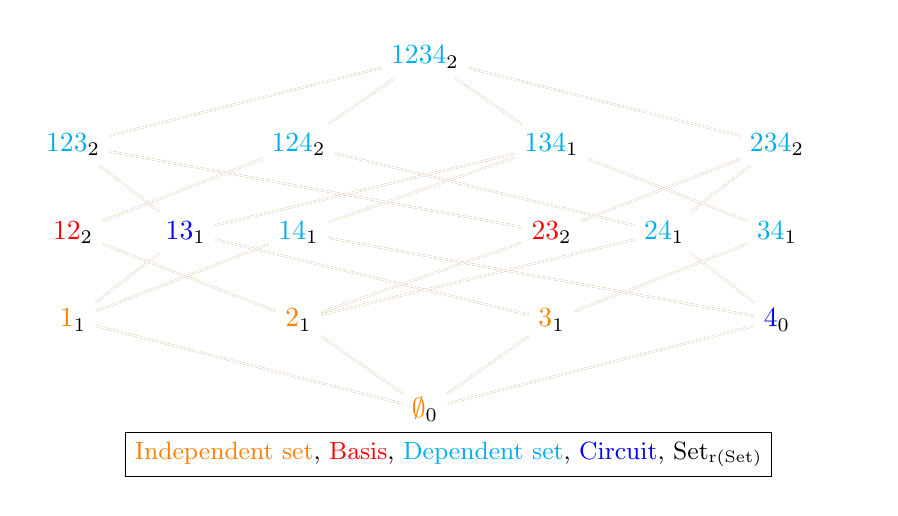
\begin{tikzpicture}

\matrix (a) [matrix of math nodes, column sep=0.6cm, row sep=0.6cm,]{
 & & &\textcolor{cyan}{
1234}_2 & & & &\\
 \textcolor{cyan}{
123}_2& &\textcolor{cyan}{
124}_2 & &\textcolor{cyan}{
134}_1 &  & \textcolor{cyan}{
234}_2  \\
\textcolor{red}{12}_2 & \textcolor{blue}{13}_1 & \textcolor{cyan}{14}_1 & & \textcolor{red}{23}_2 & \textcolor{cyan}{
24}_1 & \textcolor{cyan}{
34}_1 \\
\textcolor{orange}{1}_1& &\textcolor{orange}{2}_1 & & \textcolor{orange}{3}_1& & \textcolor{blue}{4}_0 \\
& & & \textcolor{orange}{\emptyset}_0 &  & & \\
&&&&&& \\};

\foreach \i/\j in {1-4/2-1, 1-4/2-3, 1-4/2-5, 1-4/2-7, 2-1/3-1, 2-1/3-2, 2-1/3-5, 2-3/3-1, 2-3/3-3, 2-3/3-6, 2-5/3-2, 2-5/3-3, 2-5/3-7, 2-7/3-5, 2-7/3-6, 2-7/3-7, 3-1/4-1, 3-1/4-3, 3-2/4-1, 3-2/4-5, 3-3/4-1, 3-3/4-7, 3-5/4-3, 3-5/4-5, 3-6/4-3, 3-6/4-7, 3-7/4-7, 3-7/4-5, 4-1/5-4, 4-3/5-4, 4-5/5-4, 4-7/5-4}
\draw[double, line width = 0.005mm, color = brown] (a-\i) -- (a-\j);

\node[draw] at (0, -2.5){\small \textcolor{orange}{Independent set}, \textcolor{red}{Basis}, \textcolor{cyan}{Dependent set}, \textcolor{blue}{Circuit}, $\text{Set}_{\rank(\text{Set})}$ };

\end{tikzpicture}
\end{center}

Now, let us prove that the rank function of a matroid satirfy these properties:

\begin{proof}
    \,
    \begin{enumerate}
        \item Since the co-domain is $\mathbb{Z}_{\geq0}$, $0\leq\rank(X)$. Since the maximal independent set contained in $X$ is... contained in $X$, the cardinality of that set must be smaller or equal to $|X|$. Thus, $0\leq\rank(X)\leq|X|$.
        \item Let $I_X$ be a minimal independent set contained in $X$, so $\rank(X)=|I_X|$. $I_X\subset X\subset Y$ implies that $I_X$ is an independent set contained in $Y$. Since $I_X$ may or may not be a maximal independent set contained in $Y$, $\rank(X)=|I_X|\leq\rank(Y)$. 
        \item We assume that $A\subset B\subset E$. Let $I_{A\cap B}$ be a maximal independent set contained in $A\cap B$. Since $A\cap B\subset A\cup B$, $I_{A\cap B}$ must be an independent set contained in $A\cup B$. Let $I_{A\cup B}$ be $I_{A\cap B}$ extended to be a \textbf{maximal} independent set contained in $A\cup B$. 
        
        Now let us take a look at $I_{A\cup B}\cap A$. Since the set is contained in $A$, (I2) tells us that $I_{A\cup B}\cap A$ is in independent set contained in $A$. Since the set may or may not be maximal in that regard, $|I_{A\cup B}\cap A|\leq \rank(A)$. Similarly, $|I_{A\cup B}\cap B|\leq \rank(B) $.
        
        $$ \rank(X)+\rank(Y) \geq |I_{A\cup B}\cap A|+|I_{A\cup B}\cap B| $$
        $$ = |(I_{A\cup B}\cap A)\cup(I_{A\cup B}\cap B)|+|(I_{A\cup B}\cap A)\cap(I_{A\cup B}\cap B)| $$
        $$ = |I_{A\cup B}\cap (A\cup B)|+|I_{A\cup B}\cap (A\cap B)| $$

        Since $I_{A\cup B}\subset A\cup B$, $I_{A\cup B}\cap(A\cup B) = I_{A\cup B}$.

        Since $I_{A\cap B}\subset I_{A\cup B}$, $I_{A\cup B}\cap (A\cap B) \supset I_{A\cap B}\cap (A\cap B) = I_{A\cap B} $. Let $e\in I_{A\cup B}\cap (A\cap B)$. Aiming for contradiction, suppose $e\notin I_{A\cap B}$. Since $I_{A\cap B}\cup e \subset I_{A\cup B} $, $I_{A\cap B}\cup e$ must be an independent set conained in $A\cap B$. This contradicts the fact that $I_{A\cap B}$ is a maximal in that regard. Thus, $e\in I_{A\cap B}$. This proves that $I_{A\cup B}\cap(A\cap B)\subset I_{A\cap B} $, which implies equality between the two sets.

        Thus,

        $$ \rank(X)+\rank(Y) \geq |I_{A\cup B}|+|I_{A\cap B}| = \rank(A\cup B)+\rank(A\cap B) $$
    \end{enumerate}
\end{proof}
One might observe that the rank of an independent set is the cardinality of the set itself. This is because the largest independent set that is contained in this independent set is ofcourse the independent set itself. With this property, we can define the set of independent sets with the three properties of the rank function.
\begin{theorem}
    Let $E$ be a finite set, and let $\rank : 2^E \rightarrow \mathbb{Z}_{\geq0}$ be a function satisfying (R1)-(R3). Let $\mathcal{I} = \{ I\subset E : \rank(I)=|I| \} $. Then $(E,\mathcal{I})$ is a matroid with $\rank$ as its rank function.
\end{theorem}
Before we prove this, let's prove this small theorem first:
\begin{theorem}
\label{rankextension}
    Let $E$ be a finite set and $\rank:2^E\rightarrow \mathbb{Z}_{\geq0}$ be a function satisfying (R2) and (R3). Let $X,Y\subset E$. Then if for all $y\in Y-X$, $\rank(X\cup y)=\rank(X)$, then $\rank(X\cup Y)=\rank(Y)$.
\end{theorem}
\begin{proof}
    We will prove that the statement holds with $Y-X = \{a_1,a_2,\dots,a_k\}$ holds for all itegers $k$.
    \begin{enumerate}
        \item Base case: $k=1$

        If $\rank(X\cup a_1)=\rank(X)$, then $\rank(X\cup Y)=\rank(X\cup(Y-X))=\rank(X\cup a_1)=\rank(X)$.
        \item Induction Step: Assume the statement holds for $k=n$.
        \item Let $k=n+1$: Assume that $Y-X=\{a_1,\dots,a_{n+1}\}$ for all $i\in\{1,\dots,n+1\}$ $\rank(X\cup a_i)=\rank(X)$. Then, using the assumption and our induction assumption, 
        $$ \rank(X)+\rank(X) = \rank(X\cup \{a_1,\dots,a_n\})+\rank(X\cup a_{n+1}) $$
        Using (R3), we get
        $$ \geq \rank([X\cup\{a_1,\dots,a_n\}]\cup [X\cup a_{n+1}]) + \rank([X\cup\{a_1,\dots,a_n\}]\cap [X\cup a_{n+1}]) $$
        $$ = \rank(X\cup\{a_1,\dots,a_{n+1}\}) + \rank(X) $$
        Using (R2), we get
        $$ \geq \rank(X)+\rank(X) $$
        Since $\rank(X)+\rank(X)$ is on both sides, equality holds throughout. Thus, $\rank(X\cup\{a_1,\dots,a_{n+1}\})=\rank(X\cup Y)=\rank(X)$. And thus, the statement holds for $k=n+1$.
    \end{enumerate}
    Thus, by mathematical induction, the statement holds for all integers $k$.
\end{proof}
Finally, we can prove Theorem 5:
\begin{proof}
    To prove that $(E,\mathcal{I})$ is a matroid, we will check if $\mathcal{I}$ satisfies (I1)-(I3).
    \begin{enumerate}
        \item (R1) tells us that $0\leq\rank(\emptyset)\leq|\emptyset|=0$, which implies that $\rank(\emptyset)=0=|\emptyset|$, which means that $\emptyset\in\mathcal{I}$, so (I1) is satisfied.
        \item Assume we have $J\subset I\in\mathcal{I}$. Then, using (R3),
        $$ \rank(J)+\rank(I-J) \geq \rank(J\cup[I-J])+\rank(J\cap[I-J]) = \rank(I)+\rank(\emptyset)=|I| $$
        Using (R2), we also get that
        $$ \rank(J)+\rank(I-J) \leq |J|+\rank(I-J) \leq |J|+|I-J| = |I| $$
        This implies that equality must hold throughout. At last, we show that
        $$ \rank(J)+\rank(I-J) = |J|+\rank(I-J) \Rightarrow \rank(J)=|J| $$
        Thus, $J\in\mathcal{I}$, so {I2} is satisfied.
        
        \item Suppose (I3) does not hold for some $I,J\in\mathcal{I}$ with $|I|>|J|$. Then for all $e\in I-J$, $J\cup e\notin \mathcal{I}$. Also, remember that $I,J\in\mathcal{I}$ means that $\rank(I)=|I|$ and $\rank(J)=|J|$.

        Since $J\subset J\cup e$, we can use (R1) and (R2) to see that
        $$ |J|=\rank(J)\leq\rank(J\cup e)|\leq|J\cup e|=|J|+1 $$
        $J\cup e\notin \mathcal{I}$ tells us that $\rank(J\cup e)\neq|J\cup e|$, so that must mean that $\rank(J\cup e)$ is equal to what's on the left hand side, so $\rank(J)$.

        This gives us that for all $e\in I-J$, $\rank(J\cup e)=\rank(J)$, which, according to Theorem 6, implies that $\rank(J\cup I)=\rank(J)=|J|$. However, since $I\subset J\cup I$, (R2) tells us that $\rank(J\cup I) \geq \rank(I) = |I|$, which means that $|J|\geq|I|$. This contradicts our assumption that $|J|<|I|$. Thus, (I3) is satisfied.
    \end{enumerate}
    Thus, $(E,\mathcal{I})$ is a matroid.
\end{proof}

\begin{exmp}
    

We will consider the uniform matroid $U_{2,4}$ and show that it is $\mathbb{F}_3$-representable, while it is not $\mathbb{F}_2$-representable. First, we note that $U_{2,4}= (\{1,2,3,4\}, \mathcal{I})$ where the bases are all of the two element subsets of $\{1,2,3,4\}$. So the matroid looks like: 



\begin{figure}[h]\label{u24}

\begin{center}

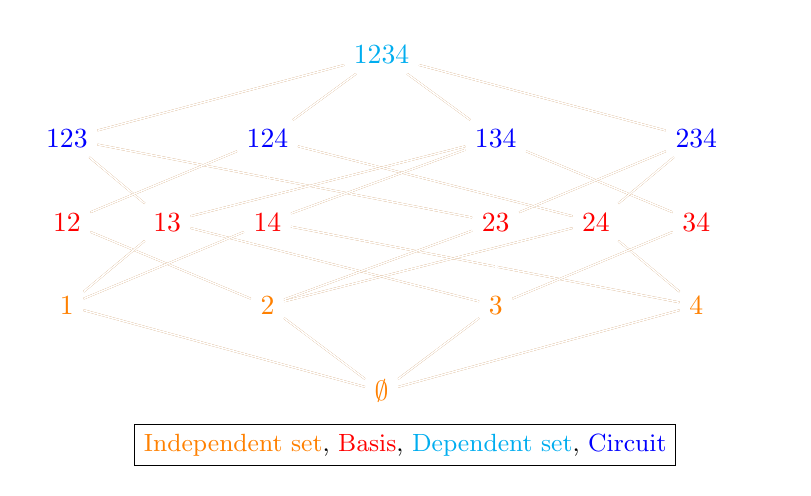
\begin{tikzpicture}

\matrix (a) [matrix of math nodes, column sep=0.6cm, row sep=0.6cm,]{
 & & &\textcolor{cyan}{
1234} & & & &\\
 \textcolor{blue}{
123}& &\textcolor{blue}{
124} & &\textcolor{blue}{
134} &  & \textcolor{blue}{
234}  \\
\textcolor{red}{12} & \textcolor{red}{13} & \textcolor{red}{14} & & \textcolor{red}{23} & \textcolor{red}{
24} & \textcolor{red}{
34} \\
\textcolor{orange}{1}& &\textcolor{orange}{2} & & \textcolor{orange}{3}& & \textcolor{orange}{4} \\
& & & \textcolor{orange}{\emptyset} &  & & \\
&&&&&& \\};

\foreach \i/\j in {1-4/2-1, 1-4/2-3, 1-4/2-5, 1-4/2-7, 2-1/3-1, 2-1/3-2, 2-1/3-5, 2-3/3-1, 2-3/3-3, 2-3/3-6, 2-5/3-2, 2-5/3-3, 2-5/3-7, 2-7/3-5, 2-7/3-6, 2-7/3-7, 3-1/4-1, 3-1/4-3, 3-2/4-1, 3-2/4-5, 3-3/4-1, 3-3/4-7, 3-5/4-3, 3-5/4-5, 3-6/4-3, 3-6/4-7, 3-7/4-7, 3-7/4-5, 4-1/5-4, 4-3/5-4, 4-5/5-4, 4-7/5-4}
\draw[double, line width = 0.005mm, color = brown] (a-\i) -- (a-\j);

\node[draw] at (0, -2.5){\small \textcolor{orange}{Independent set}, \textcolor{red}{Basis}, \textcolor{cyan}{Dependent set}, \textcolor{blue}{Circuit} };

\end{tikzpicture}
\end{center}
\caption{Representation of $U_{2,4}$}

\end{figure}

Suppose $U_{2,4}$ were $\mathbb{F}_2$-representable. Then there is some $A = \mat_{m \times 4}(\mathbb{F}_2)$, 

$$A = \begin{pmatrix}
    v_1 & v_2 & v_3 & v_4
\end{pmatrix}$$

so that $U_{2,4} \sim M[A]$. We have the following observation.

\begin{lemma}
\label{f2lema}
    Suppose a set of vectors $A = \{w_1, w_2, \cdots, w_r\} \subseteq \mathbb{F}_2^n$ is minimaly linarly dependent, that means that it is linarly dependent but any proper subset of it is linearly independent. Then $w_1 + w_2 + \cdots + w_r = 0$.
\end{lemma}

\begin{proof}
    Because $A$ is linearly dependent, there exists a set of scalars $\{a_1, a_2, \cdots, a_r\}\in \mathbb{F}_2$ not all zero such that
    
    $$\sum_{i=1}^r a_iv_i = 0.$$
    
    If for some $1\leq j \leq r$ we have $a_j = 0$ then we also have 
    
    $$\sum\limits_{\substack{i = 1 \\ i \neq j}} ^r a_iv_i = 0$$

    but not all out of $a_1, \cdots a_{j-1}, a_{j+1}, \cdots a_r$ are 0. This means that ${v_1, \cdots, v_{j-1}, v_{j+1}, \cdots, v_r}$ is linearly dependent, which is not true by assumption. Therefore, for all $1\leq j \leq r$ we have $a_j \neq 0$. But since the field is $\mathbb{F}_2$ this forces $a_j = 1$ for all $j$. Hence, we obtained what we want, namely

     $$\sum_{i=1}^r a_iv_i = 0 =  \sum_{i=1}^r 1 \cdot v_i = 0.$$
    
\end{proof}

If the matroid $U_{2,4} \sim M[A]$ for the above $A$ then we would have all of the three element subsets of vectors to be minimally linearly dependent. This means by lemma(\ref{f2lema}) that $v_1 + v_2 + v_3 = 0$ and $v_1 + v_2 + v_3 = 0$. However, we are in $\mathbb{F}_2$ so 


$$v_1 + v_2 + v_3 = 0 \iff v_1 + v_2 + (v_3 + v_3) = v_3 \iff v_1 + v_2 = v_3 $$

And in the same way $v_1 + v_2 = v_4$. This implies that
$$v_3 + v_4 = (v_1 + v_2 )+ (v_1 + v_2) = 0$$
so the set $\{v_3, v_4\}$ is linearly dependent, which is a contradiction. So $U_{2,4}$ is not $\mathbb{F}_2$-representable. However, $U_{2,4}$ is $\mathbb{F}_3$-representable. For instance the following matrix taken from \cite[20]{oxley1} works, namely

$$A = \begin{pmatrix}
    1 & 0 & 1 & 1 \\
    0 & 1 & 1 & 2
\end{pmatrix}$$.

 We see that no column vector of $A$ is 0, so all single-element subsets are independent. No vector is a scalar multiple of each other, so two element subsets are independent. Finally, no 3-element subsets can be independent, since the dimension of the $\mathbb{F}_3^2$ is 2, so the dimension of any subspace is at most 2.

To conclude the example of $U_{2,4}$, we will show that $U_{2,4}$ has an interesting property that it is not a graphic matroid. In other words, we can show that there is no graph $G$ such that $U_{2,4} \sim M$ where $M$ is the matroid formed by the set of edgs of $G$ with the usual rules. 

We will show $U_{2,4}$ is not graphic by contradiction, that is assume $U_{2,4}$ is graphic and let $G$ be the graph it represents. Then $G$ has four edges and since all two-element subsets of $U_{2,4}$ are independent we see that $G$ has no loops or parallel edges. In particular, all three-element subsets of $U_{2,4}$ are circuits, so in the graph the edges they correspond to form a cycle. But if both sets $\{1,2,3,\}$ and $\{1,2,4\}$ corresonds to edge cycles without parallel edegs it immediatly follows that $3$ and $4$ connect the same vertices, i.e. are parallel edges, which is a contradiction. It follows that $U_{2,4}$ is not graphic.

%In the succeeding sections, we will also consider an example of a matroid, which is not representable over any field.

\end{exmp}





%\input{graphic} already inside definitions



\newpage
\section{Closure Operator}


We will introduce one more important notion, the one of closure operator. As the name 'operator' suggests, it is a map between objects of the same type. Our objects are, of course, the subsets of the ground set of a matroid. The idea of the closure operator is that it adds to any subset $X \subseteq E$ whatever is left in $E$ that does not change the rank when added to $X$. In doing so it will produce \textit{closed sets} which are in matroid theory called flats, another collection of subsets with distinctive properties. 

Closure also has interesting interpretation in the case of our main examples of representable and graphic matroids. In the case of representable matroids, it adds to $X$ all elements which are in the vector span of $X$ and contained in $E$ (thus it will not increase the vector rank of $E$). In the case of graphic matroids it will add to any set of edges, all edges that create cycles between its sets of vertices (thus will not increase the size of the spanning forest).

\begin{defn}
    Let $M = (E, \mathcal{I})$ be a matroid. The closure operator is a function $\cl: 2^E \to 2^E$ such that

    $$\cl(X) = \{x \in E\; | \; \rank(X \cup x) = \rank(X) \}.$$

    
\end{defn}

The operator has numerous important properties. This time we will immediately prove the reverse statement. Namely, that these characteristic properties \textit{uniquely characterize} the closure operator of a matroid.

\begin{theorem}
Let $M = (E, \mathcal{I})$ be a matroid and $\cl: 2^E \to 2^E$ be a function. Then $\cl$ is the closure operator of $M$ if and only if

\begin{enumerate}
    \item[(CL1)] For any $X \subseteq E$ we have $X \subseteq \cl (X)$.
    \item[(CL2)] If $X \subseteq Y \subseteq E$ then $\cl(X) \subseteq \cl(Y)$.
    \item[(CL3)] For all $X$ we have $\cl(\cl(X)) = \cl(X)$.

    \item[(CL4)] Let $X \subseteq E$ and $b \in 
    \cl(X \cup a) - \cl(X)$ then $a \in \cl(X \cup b)$.
\end{enumerate}
\end{theorem}


\begin{proof}
    All the four statements in the \textit{only if} direction (assuming $\cl$ is the closure operator) are rather straightforward, and we will prove them first. 
    
    \begin{enumerate}
     
    \item[$\implies$]  
    We first assume $\cl$ is the closure operator and would like to show the four properties.
    
        \begin{enumerate}
            \item[(CL1)] If $X\subseteq E$ is arbitrary, and we pick any element $x \in X$ then $X \cup x = X$. Consequently, $r(X \cup x)= r(X)$ thus $x \in \cl(X)$ by definition of the closure operator which shows the inclusion $X \subseteq \cl(X)$.
    
            \item[(CL2)] Let $X \subseteq Y \subseteq E$
            and $x \in \cl(X)$. This is equivalent to saying $\rank(X \cup x) = \rank(X)$. Because we would like to show that $x \in \cl(Y)$ we would by definition like that $\rank(Y \cup x) = \rank(Y).$ In particular, we observe that we can without loss of generality assume $x \in \cl(X) - Y$ since the result trivially follows if $x$ is already in $Y$. 
            
            This immediately incentivizes us to check some rank function inequalities containing the sets $X, Y - X$ and these sets containing $x.$ In particular, it would be good if we would come to the inequality 
            $\rank(Y\cup x) \leq \rank(Y)$.
            So our goal is to choose a suitable set $A$ such that $Y \cup A = Y \cup x$ while $\rank(Y \cap A) = \rank(A)$ and we could use the inequality of the rank function (R3). More specifically, what we would like is
    
            $$\rank(\underbrace{Y \cup A}_{ = Y  \cup x}) + \underbrace{\rank(Y \cap A)}_{ = \rank(A)} \leq \rank(Y) + \rank(A).$$
    
            One $A$ that does exactly this is $A = X \cup x.$ Then we have, since $X \subseteq Y$ that $Y \cup A = Y \cup X \cup x = Y \cup x$, and since we are assuming $x \in \cl(X) - Y$ we have $Y \cap (X \cup x) = X $.
    
            So $$\rank(Y\cup (X \cup x)) + \rank(X) \leq \rank(Y) + \rank(X \cup x),$$ and since $\rank(X \cup x) = \rank(X)$ by assumption, we have 
            $\rank(Y \cup x)\leq \rank(X)$ what we wanted to show. To conclude, the inequality $\rank(Y) \leq \rank(Y \cup x)$ follows by (R2) so we have $\rank(Y) \leq \rank(Y\cup x) \leq \rank(X)$ implying $\rank(Y \cup x ) = \rank(X)$ so by definition $x \in \cl(Y)$.
    
            So we have shown the inclusion $\cl(X) \subseteq \cl(Y)$ which was our goal.
    
            \item[(CL3)] By combining the first and the second property already of closure we have already proven, the inclusion $\cl(X) \subseteq \cl(\cl(X))$  follows. We have to exhibit the reverse one as well, so suppose $z\in \cl(\cl(X))$. This means $\rank(\cl(X) \cup z)= \rank(\cl(X))) = \rank(X)$ where the last inequality follows by the theorem (\ref{rankextension}), namely for all $v \in \cl(X)$ we by definition have $\rank(X \cup v) = \rank(X)$ so by theorem (\ref{rankextension}) we have $\rank(\cl(X)) = \rank(X)$. But now we have, since $X \subseteq \cl(X)$ that $$\rank(X) \leq \rank(X \cup z) \leq \rank(\cl(X)\cup z) = \rank(X),$$
    
           therefore, the equality holds in all inequalities above. In particular, this means that $\rank(X \cup z) = \rank(X)$ which by definitions means that $z \in \cl(X)$. So the desired inclusion $ \cl(\cl(X))\subseteq \cl(X)$ also holds, which finally implies the desired equality of sets $\cl(\cl(X))= \cl(X).$
    
            \item[(CL4)] Let $X \subseteq E$ be arbitrary and $b \in \cl(X \cup a) - \cl(X)$. Since, $b \in \cl(X \cup a)$ we have $\rank((X\cup a)\cup b) = \rank((X\cup b) \cup a) = \rank(X \cup a)$ by definition. 
    
            Now since $b \notin \cl(X)$ then by definition $\rank(X \cup b)\neq \rank(X)$, and because $X \subseteq X \cup b$ we have by (R2) that $\rank(X \cup b) > \rank(X)$. In particular, since the rank function measures the size of the largest independent set inside a given subset, adding an element to a set can increase its rank by at most 1, so we have that $\rank(X \cup b) = \rank(X)+1.$ 
    
            Now since $\rank(X \cup a \cup b) = \rank(X \cup a)$, and by the same reason as in the previous paragraph, since $\rank(X \cup a)$ is either $\rank(X)$ or $\rank(X) + 1$, we have it is, in fact, equal to $\rank(X) + 1$ since $\rank(X \cup a) = \rank(X \cup a \cup b) \geq \rank(X \cup b)= \rank(X) + 1$.
    
            So we have $r((X\cup b) \cup a) = \rank(X \cup b)$ or in other words, $a \in \cl(X \cup b)$ by definition, which is precisely what we wanted to show.
           
            \end{enumerate}
    


    \item[$\impliedby$] Now we prove the more complicated reverse direction. We assume we have a finite set $E$ and an arbitrary function $\beta : 2^E \to 2^E$ satisfying the properties of the closure operator listed above.

    Unlike the proofs of the reverse implication of the cryptomorphisms in terms of bases, circuits or rank function, where we had a very straightforward way to spot where the independent sets should appear (for bases they are all of the subsets of members of $\mathcal{B}$, for circuits they are all sets which contain no members of $\mathcal{C}$ and for the rank function they are sets with the property that $\rank(X) = |X|$), this is now not the case, or is at least not immediately apparent.

    So we will not relate the function $\beta$ directly to the independent sets, but rather some other cryptomorphic definition of matroids we have already proven. In particular, observe that if $\cl(X) = E$ holds for some subset $X \subseteq E$ this means that the rank of $X$ is $r(E)$, or in other words, the maximal independent set inside of $X$ is a \textit{basis.}

    Therefore our goal is to look at the collection of all subsets such that $\beta(X)= E$ and prove that the subcollection of its \textit{minimal sets} satisfies the axioms for the collection of bases of a matroid. The following proof is our own, in \cite[p. 27]{oxley1}, the author manages do define independent sets purely in terms of the closure, but we find our proof more intuitive, so we will present here. Therefore, we define $\mathcal{B}' = \{X \subseteq E\; |\; \beta(X) = E\;\}$ and call $\mathcal{B}$ the collection of minimal members of $\mathcal{B}$, for reminder, that are sets which are in $\mathcal{B}$ but do not contain any members of $\mathcal{B}$ as their proper subsets.


\begin{enumerate}

\item[(B1)] We have to prove that $\mathcal{B}$ satisfies the two basis axioms. The first one (B1) is evident since by the first property of closure operator we have the first inclusion in $E\subseteq\beta(E) \subseteq E$ and the second follows because $\beta$ maps into $2^E$. So $E \in \mathcal{B}'$ which in particular implies that $\mathcal{B}'$ and consequently $\mathcal{B}$ are nonempty.

\item[(B2)]
    For the second property (B2) assume $B_1, B_2$ are distinct elements of $\mathcal{B}.$ Because $\mathcal{B}$ consists of \textit{minimal} sets we know that if they are distinct one cannot be a subset of another. So let us pick any $x \in B_1 - B_2$.
    We observe two things, first, $\beta(B_1) = E$ and $\beta(B_1 - x) \neq E$ since $B_1$ is minimal. It is also clear that there exists $y \in B_2 - B_1$ such that $y \in E - \beta(B_1 - x)$, this is because, otherwise all the elements of $B_2$ would be in $\beta(B_1-x)$, but then we would have that $B_2 \subseteq \beta(B_1 - x)$ by (CL2) we would have that $E = \beta(B_2)\subseteq \beta(\beta(B_1 - e)) = \beta(B_1 - e) \neq E$. So by (CL4) we have that we can exchange $x$ and $y$ in the following inclusion.
    
    $$y \in E - \beta(B_1 - x) = \beta((B_1 -x )\cup x)-\beta(B_1 - x)$$ which directly implies that $x \in \beta((B_1 - x)\cup y)$. Now we are done, because this means that 
    
    $$\beta((B_1-x)\cup y) = \beta(\beta((B_1-x )\cup y)) = \beta(\beta((B_1 - x)\cup y)\cup x) \supset \beta(B_1) = E,$$
    
    
    where we have used (CL3) in the first equality and $x\in \beta((B_1-x)\cupy)$ in the second equality. Thus, $(B_1 - x) \cup y$ is in $\mathcal{B}'$ by definition, since its $\beta$ is $E$. We still have to show that $(B_1 - x)\cup y$ is minimal.
    
    Therefore, we will prove separately that all the members of $\mathcal{B}$ have the same size. Let $B_{min}$ be a member of $\mathcal{B}$ with the smallest size and $B_3$ a member of $\mathcal{B}$ such that among all such possible pairs ($B_{min}$ has the smallest number of elements and $B_3$ is another member of $\mathcal{B}$ not equal to $B_{min}$) we have that $|B_{min} \cap B_3|$ is maximal. Since both elements are minimal members of $\mathcal{B}'$ they are not subsets of each other. In particular, this means we can choose $x \in B_{min} - B_3$. 
    
    We know that $\beta(B_{min}-x) \neq E$ and what is more, by the similar argument as before, there has to be $y \in B_3 - \beta(B_{min} - x)$, since otherwise $B_3 \subseteq \beta(B_{min} - x)$ which would mean that $E = \beta(B_3)\subseteq \beta(\beta(B_{min}-x)) = \beta(B_{min} - x)$ which is a contradiction. 
    
    So we have that $y \in \beta((B_{min}-x)\cup x) - \beta(B_{min} -x)$ and (CL4) we thus have $x \in \beta((B_{min}-x)\cup y)$ - we exchange $x$ and $y$. 
    
    However, we see two things. First
    $$\beta((B_{min} - x) \cup y) \supset \beta(B_{min}) = E,$$ so $(B_{min} - x) \cup y \in \mathcal{B}'$ and $|B_{min}|  = |(B_{min} - x)\cup y|$ so $(B_{min} - x)\cup y$ is a member of $\mathcal{B}'$ with the smallest possible number of elements. 
    
    Second we see that $|((B_{min}-x)\cup y) \cup B_3| = |B_{min}\cup B_3|+1$ which contradicts the maximality of pair $(B_{min} ,B_3)$. 
    
    So all the elements of $\mathcal{B}$ have the same size, which in  particular implies that $(B_1 - x) \cup y \in \mathcal{B}$ since it is $\beta$  is $E$ what we wanted to show.
    

\end{enumerate}


\end{enumerate}

The last thing to check is if $\beta$ is, in fact, the closure operator for the matroid with the basis set $\mathcal{B}.$ We first introduce some notation, let $M = (E, \mathcal{I})$ be the matroid we are interested in, meaning the one with the basis set $\mathcal{B}$ and we denote its rank function by $\rank'$ and its closure operator by $\cl'$. Our goal is to show that for all subsets $X$ we have that $\cl'(X) = \beta(X)$, i.e. the operators coincide.

We know that $\beta$ and $\cl'$ already do coincide on some sets, precisely the ones that contain a basis, for such $X$ we have $\beta(X) = \cl'(X) = E.$

Second thing to note is that $\beta$ preserves rank, i.e., we always have $\rank'(\beta(X)) = \rank'(X)$ for all $X\subseteq E$. We will prove this by contradiction, let $\rank'(M) = n$. Suppose there is some subset $X$ with $k  = \rank'(X)<\rank'(\beta(X)) = l$ (applying $\beta$ to $X$ has to increase the rank because $X \subseteq \beta(X)$). Then the largest independent set $L$ of $\beta(X)$ has the size $l$. We know $L$ is in some basis $B$ of $\mathcal{B}$, i.e. $L \subseteq B$. Let us observe the set $X \cup (B-L)$.  Its largest independent set has the size at most $k + (n-l)<n$, because the largest independent set of $X$ has size $k$ and we added $|B-L| = n - l$ elements to it, so we increase it by at most $n-l$. The point is that because $k<l$ we have $k + (n-l)<n$, which in particular means that \textit{there is no basis} in $X \cup (B-L)$ and that its rank is less than $n.$


But on the other hand, we have

$$L \subseteq \beta(X) \subseteq \beta(X \cup (B-L))$$ and $$B-L \subseteq \beta(X \cup (B-L))$$ which in particular means that $B \subseteq \beta(X \cup (B-L))$. Finally, this would mean that  
$E = \beta(B)\subseteq \beta(\beta(X \cup (B-L))) = \beta(X \cup (B-L))$ which would imply, by definition of $\mathcal{B}$ that $X \cup (B-L)
\in \mathcal{B}$ - which ultimately means it \textit{contains a basis} of our matroid. But we have already established this is not the case, so we have come upon a contradiction. Therefore, $\beta$ preserves rank.
The fact that $\beta$ preserves rank and looking at the definition of the closure operator, namely that it puts in all the elements which preserve rank, we have thus obtained the inclusion $\beta(X) \subseteq \cl'(X)$ for all subsets $X.$

Finally, suppose for contradiction that for some $X$ the latter inclusion $\beta(X) \subseteq \cl'(X)$ is proper and additionally assume that $X$ is a maximal set with these properties (at some point this will have to stop since for $X =E$ the equality $\beta(E) = \cl'(E) = E$ holds.) First, we pick $x \in E - \cl'(X)$ such that $\cl'(X\cup x) - \cl'(X)$ is nonempty (there exists such an $x$ because $X$ does not contain a basis, otherwise, the equality $\beta(X) = \cl'(X) = E$ would hold).
Because of the maximality of $X$ we hence know that $\beta(X\cup x) = \cl'(X \cup x)$ holds. Also, since the inclusion $\beta(X) \subseteq \cl'(X)$ is proper, we can pick $r \in \cl'(X) - \beta(X)$. In particular, we then have that $r \in \beta(X\cup x) - \beta(X)$ so by (CL4) we have $x \in \beta(X\cup r)$.

However, this means that $X \cup x \subseteq \beta(X\cup r)$ and since $X\cup r \subseteq \cl'(X)$ we have that $\rank'(X\cup r) = 
\rank'(X)$. But on the other hand $$\rank'(X) + 1= \rank'(X\cup x) = \rank'(\beta(X\cup x))\leq \rank'(\beta(\beta(X\cup r))) = \rank'(\beta(X\cup r)) = \rank'(X\cup r) = \rank'(X)$$

which is a contradiction. So our initial assumption that the inclusion $\beta(X) \subseteq \cl'(X)$ is proper for some $X$ was false, which implies that $\beta(X) = \cl'(X)$ for all $X$ and we are done.

\end{proof}


With the definition of closure operator we can define three more important family of subsets of a matroid.

\begin{defn}\label{HP&SS}
    Let $M = (E, \mathcal{I})$ be a matroid with the rank function $\rank$ closure operator $\cl.$ We call a subset $X \subseteq E$ a flat if $\cl(X) = X$ holds. We call a subset $H \subseteq E$ a hyperplane if $H$ is a rank with $\rank(H) = \rank(E)-1$. Finally, we call a subset $S \subseteq E$ a spanning set if $\cl(S) = E$.
\end{defn}



\section{Flats}

In \cite[35]{oxley1} we have as an excercise an alternative characterization of matroids in terms of their flats. Because we think it is a prototypical model of a statement of the form (a collection of subsets satisfies properties X) if an only if ( it is some well known family of matroid subsets) we will show our proof here.

    Given a matroid $M$ with a ground set $E$ and its collection of flats, that is all the subsets $X \subset E$ satisfying $\cl(X) = X$, the statement 'abstracts out' which properties of flats \textit{make them flats}. Such statements are a common theme of our article.

\begin{theorem}
    Let $M = (E, \mathcal{I})$ be a matroid. A collection $\caf$ is a collection of flats if and only if the following three conditions hold

    \begin{enumerate}
        \item We have $E \in \caf$.
        \item If $F_1, F_2 \in \caf$ then $F_1 \cap F_2 \in \caf$.
        \item If $F \in \caf$ and $\{F_1, F_2, \cdots, F_k\}$ is a collection of all minimal members of $\caf$ properly containing $F$ then $\{F_1-F, F_2-F, \cdots, F_k - F\}$ partition $E-F$.
        
    \end{enumerate}
        
\end{theorem}

As an example, we can once again return to our depiction from earlier. This time, we write flats in cursive and with a line below it. As one can see, every superset of a flat has a larger rank. One can see here that the ground set is indeed a flat, and the intersection of for example \textit{134} and \textit{24} is indeed another flat, \textit{4}. In this picture, only dependent sets are flats. However, if all supersets one larger than a certain independent set are also independent, then that independent set is a flat. We unfortunately do not have such a situation in this matroid. 

\begin{center}
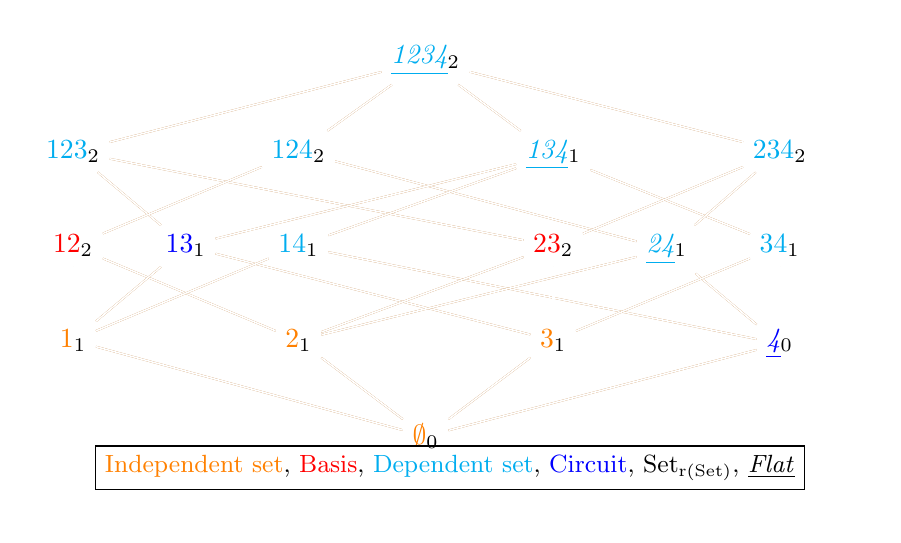
\begin{tikzpicture}

\matrix (a) [matrix of math nodes, column sep=0.6cm, row sep=0.6cm,]{
 & & & \textcolor{cyan}{\underline{\textit{1234}}}_2 & & & &\\
 \textcolor{cyan}{
123}_2& &\textcolor{cyan}{
124}_2 & &\textcolor{cyan}{\underline{\textit{134}}}_1 &  & \textcolor{cyan}{
234}_2  \\
\textcolor{red}{12}_2 & \textcolor{blue}{13}_1 & \textcolor{cyan}{14}_1 & & \textcolor{red}{23}_2 & \textcolor{cyan}{\underline{\textit{24}}}_1 & \textcolor{cyan}{
34}_1 \\
\textcolor{orange}{1}_1& &\textcolor{orange}{2}_1 & & \textcolor{orange}{3}_1& & \textcolor{blue}{\underline{\textit{4}}}_0 \\
& & & \textcolor{orange}{\emptyset}_0 &  & & \\
&&&&&& \\};

\foreach \i/\j in {1-4/2-1, 1-4/2-3, 1-4/2-5, 1-4/2-7, 2-1/3-1, 2-1/3-2, 2-1/3-5, 2-3/3-1, 2-3/3-3, 2-3/3-6, 2-5/3-2, 2-5/3-3, 2-5/3-7, 2-7/3-5, 2-7/3-6, 2-7/3-7, 3-1/4-1, 3-1/4-3, 3-2/4-1, 3-2/4-5, 3-3/4-1, 3-3/4-7, 3-5/4-3, 3-5/4-5, 3-6/4-3, 3-6/4-7, 3-7/4-7, 3-7/4-5, 4-1/5-4, 4-3/5-4, 4-5/5-4, 4-7/5-4}
\draw[double, line width = 0.005mm, color = brown] (a-\i) -- (a-\j);

\node[draw] at (0, -2.5){\small \textcolor{orange}{Independent set}, \textcolor{red}{Basis}, \textcolor{cyan}{Dependent set}, \textcolor{blue}{Circuit}, $\text{Set}_{\rank(\text{Set})}$, \underline{\textit{Flat}} };

\end{tikzpicture}
\end{center}

\begin{proof}
Before we begin the proof, we have two notable observations. First, we see that the characterization of our collection $\caf$ follows a similar pattern as characterization of other encountered collections such as $\mathcal{I}$ or $\mathcal{C}$. Specifically, we mean that we have two initializing properties, for example, the collection is non-empty, has $\emptyset$ or $E$, is downard closed, closed under intersections, inclusions... Followed by the third property which really tells us something non-trivial about how the sets of the collection interect with each other. 
Second, as with the previous proofs, we will see that it is not hard to prove the only if direction, i.e. knowing we have a collection of flats and proceeding further. However, we will require some clever ideas to prove the reverse direction.

So first suppose $\caf$ is a collection of flats and our goal is to prove that the three properties hold. 

\begin{enumerate}
    \item We see that $E \subset \cl(E)$ by the definition of the closure operator and $\cl(E)\subset E$ because $\cl$ maps from $2^E$ into $E.$ Thus $\cl(E)= E$ implying $E$ is a flat as desired.
    
    \item Again, inclusion $F_1 \cap F_2 \subset \cl(F_1 \cap F_2)$ is a fundemental property of closure operator (CL1). Because $F_1 \cap F_2 \subset F_1$ we have by (CL2) that $\cl(F_1 \cap F_2) \subset \cl(F_1) = F_1$ where the last equality follows by assumption that $F_2$ is a flat. Similarly $\cl(F_1\cap F_2) \subset F_2$, which implies $\cl(F_1\cap F_2)$ is contained in $F_1$ and $F_2$, in other words $\cl(F_1 \cap F_2) \subset F_1 \cap F_2$. To conclude $F_1 \cap F_2 \subset \cl(F_1 \subset F_2) \subset F_1 \cap F_2$ which implies $\cl(F_1 \cap F_2) = F_1 \cap F_2$, and then by definition $F_1 \cap F_2 \in \caf$ thus the second property is satisfied.

    \item We pick a flat $F$ and let $P = \{F_1, F_2, \cdots, F_k\}$ be the collection of all flats properly containing $F$. To show that $P$ partitions $E - F$ we have to show two things; for any $i \neq j$ we must have $(F_i - F)\cap( F_j - F) = \emptyset$ and $\cup_{k}( F_k - F) = E - F.$ 
    
    The second property is evident, namely if we pick any $x \in E - F$ then there exists a flat containing $F \cup x, $ in particular $E$ will do. So there exists a minimal (not properply containing other with such properties) flat containing $F \cup x$, let us call it $G$ and obviously, $G = \cl(F \cup x)$. We would like $G$ to also be a minimal flat properly containing $F$. If it is not there is some flat $H$ such that $F \subset H \subset G$ where both inclusions are proper. By assumption $H$ does not include $x$ otherwise it would contradict the minimality of $G.$ But there also has to be some $y \in H - F$. In particular, since all things involved are flats, we have that $y \in \cl(F \cup x) - \cl(F)$ so by (CL4) we have $x \in \cl(F \cup y)$ which is a contradiction since $\cl(F \cup y)$ is a flat which contains $F$ and $y$ so it is $H.$  Therefore $G$ is a minimal flat and we are done.

    The first property can be derived by contradiction. Namely, if for some $i\neq j$ we have that there exists $e \in (F_i - F)\cup(F_j - F)$ then we have that the intersection $F_i \cup F_j$ is a flat which contains $F\cup e$, but is also properly contained inside $F_j$ and $F_i$ - a contradiction.

    So we also have the last property.
    
\end{enumerate}

    Now for the if direction. In the previous proofs of proving the reverse direction of such statements we could directly relate the independent sets, which we consider to be our most elementary definition, to our objects. For example if you know your collection has to be the collection of circuits, then the independent sets are precisely all of the proper subsets of circuits. If you know your collection has to be a collection of bases, then the independent sets have to be all of their subsets. When proving the equivalence of the rank function, the independent sets were precisely the sets with the propery $r(X) = |X|$. 

    However, with flats, there is no way (at least not as clear as with previous examples) to relate flats with independent sets. So we will prove the reverse direction by relating it to one definition we already know. So we have to prove that $f$ satisfies the properties (CL1) - (CL4).

    Suppose we are given a finite set $E$ and collection $\caf$ of its subsets satisfying properies 1., 2. and 3. Then let us define a \textit{function} $f: 2^E \to \caf$ by the rule that for any $X$, we have $f(X)$ is the minimal member of $\caf$ containing $X$. Its clear what is our aim, namely to show that this is in fact a closure operator, then we will do two things at once - $E$ will be a matroid with a closure operator $f$ and the elements of $\caf$ will be precisely the flats.

    First we have to check $f$ is well-defined. By the first property of $\caf$ we have that $E \in \caf$ and because for any subset $X \subset E$ we have $X \subset E$ we have that for every subset $X$ there \textit{exists} some element of $\caf$ such that $X$ is a subset of it (in the worst case it is $E$). Now, the minimal such subset has to be unique, since if $F_1, F_2$ have the same property that they are minimal members of $\caf$ including $X$ then by the second property of $\caf$ we have that $F_1 \cap F_2 \in \caf$ and so $X \subset F_1\cap F_2$, so if they are not the same we are contradicting minimality of them. $ F_1 \subset F_2$ and $F_2 \subset F_1$ hold so $F_1 = F_2.$

    Now we check the closure axioms.

\begin{enumerate}
    \item If $X \subset E$ then by definition, $f(X)$ is an element of $\caf$ \textit{containing} $X$ so we have $X \subset f(X)$ and the first property follows.
    
    \item If $X \subset Y \subset E$ then $f(X)$ is the minimal member of $\caf$ containing $X$. Because $f(Y)$ is a minimal member of $\caf$ which contains $Y$ it thus also contains $X$ so by minimality of $f(X)$ we have $f(X)\subset f(Y)$ as desired.

    \item If $X \subset E$ is arbitrary then we have that $f(f(X))$ is the minimal member of $\caf$ containing $f(X)$, but $f(X)$ is by defintion itself in $\caf$ and it contains $f(X)$. So we have that $f(X) \subset f(f(X)) \subset f(X)$ implying $f(f(X)) = f(X).$

    \item Up to this point we have not yet used the second and the third property of $\caf$ so we better require them now.

     Suppose $X \subset E$, $x \in E$ and $y \in f(X \cup x) - f(X)$. In particular, this means that $y \notin X$.
   Our goal is to show $x \in f(X \cup y)$. Let us call $f(X) = F_1$, $f(X \cup x) = F_2$ and $f(X \cup y) = F_3$ to remind us that output of $f$ is always a member of $\caf$. By the second property of "closure operator" we have already proved, we have $F_1 \subset F_2$ and $F_1 \subset F_3$. Not just that, $F_2$ and $F_3$ are in fact one of the minimal elements of $\caf$ properly containing $F_1$.

     We know this, because by the third property of $\caf$, all of the minimal elements of $\caf$ containing $F_1$ \textit{partition} $E-F_1$, so in particular, there is some $F_2' \in \caf$ which contains $X\cup x$ and contains $X$ minimaly and some $F_3' \in \caf$ which contains $X \cup y$ and contains $X$ minimally. So from $X \cup x \subset F_2' \in \caf$ we directly infer $F_2 \subset F_2'$ because $f(X \cup x)$ is an element of $\caf$ which contains $X \cup x$ minimally. It is now clear that $F_2= F_2'$ and $F_3 = F_3'$.


     We are almost done. By the third property of $\caf$, because $F_2$ and $F_3$ are minimal members of $\caf$ properly containing $X$ we have that $(F_2-F_1)\cap (F_3 - F_1)$ is either empty or $F_2 = F_3$. It cannot be empty because, $y \in F_3 - F_1$ by definition and $y \in f(X\cup x)-f(X) = F_2 - F_1$ by assumption. So $F_2 = F_3$ which implies that $x \in F_3 = f(X \cup y).$ This shows the last closure axiom, and in particular, we know that we have a matroid with ground set $E$ and closure operator $f.$


     Finally, it is clear by defnition that the collection of all subsets of $X$ such that $f(X) = X$ is precisely $\caf$, so $\caf$ is our collection of flats for this matroid.
     
\end{enumerate}


    
\end{proof}



%

We will consider the uniform matroid $U_{2,4}$ and show that it is $\mathbb{F}_3$-representable, while it is not $\mathbb{F}_2$-representable. First, we note that $U_{2,4}= (\{1,2,3,4\}, \mathcal{I})$ where the bases are all of the two element subsets of $\{1,2,3,4\}$. So the matroid looks like: 



\begin{figure}[h]\label{u24}

\begin{center}

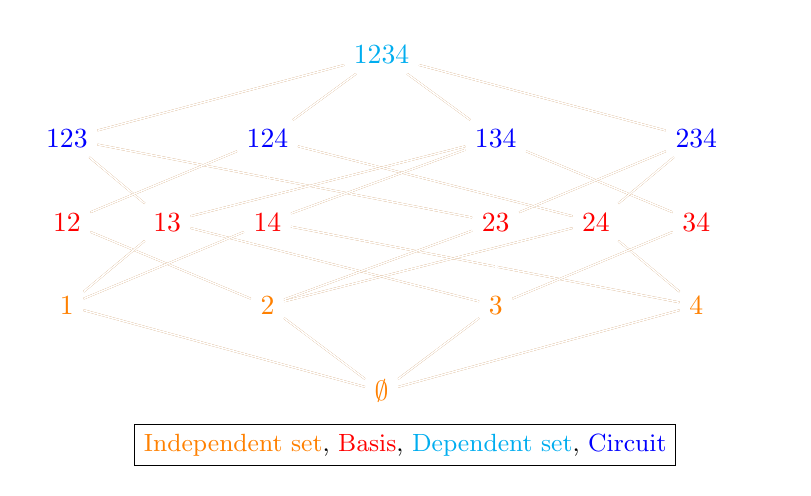
\begin{tikzpicture}

\matrix (a) [matrix of math nodes, column sep=0.6cm, row sep=0.6cm,]{
 & & &\textcolor{cyan}{
1234} & & & &\\
 \textcolor{blue}{
123}& &\textcolor{blue}{
124} & &\textcolor{blue}{
134} &  & \textcolor{blue}{
234}  \\
\textcolor{red}{12} & \textcolor{red}{13} & \textcolor{red}{14} & & \textcolor{red}{23} & \textcolor{red}{
24} & \textcolor{red}{
34} \\
\textcolor{orange}{1}& &\textcolor{orange}{2} & & \textcolor{orange}{3}& & \textcolor{orange}{4} \\
& & & \textcolor{orange}{\emptyset} &  & & \\
&&&&&& \\};

\foreach \i/\j in {1-4/2-1, 1-4/2-3, 1-4/2-5, 1-4/2-7, 2-1/3-1, 2-1/3-2, 2-1/3-5, 2-3/3-1, 2-3/3-3, 2-3/3-6, 2-5/3-2, 2-5/3-3, 2-5/3-7, 2-7/3-5, 2-7/3-6, 2-7/3-7, 3-1/4-1, 3-1/4-3, 3-2/4-1, 3-2/4-5, 3-3/4-1, 3-3/4-7, 3-5/4-3, 3-5/4-5, 3-6/4-3, 3-6/4-7, 3-7/4-7, 3-7/4-5, 4-1/5-4, 4-3/5-4, 4-5/5-4, 4-7/5-4}
\draw[double, line width = 0.005mm, color = brown] (a-\i) -- (a-\j);

\node[draw] at (0, -2.5){\small \textcolor{orange}{Independent set}, \textcolor{red}{Basis}, \textcolor{cyan}{Dependent set}, \textcolor{blue}{Circuit} };

\end{tikzpicture}
\end{center}
\caption{Representation of $U_{2,4}$}

\end{figure}

Suppose $U_{2,4}$ were $\mathbb{F}_2$-representable. Then there is some $A = \mat_{m \times 4}(\mathbb{F}_2)$, 

$$A = \begin{pmatrix}
    v_1 & v_2 & v_3 & v_4
\end{pmatrix}$$

so that $U_{2,4} \sim M[A]$. We have the following observation.

\begin{lemma}
\label{f2lema}
    Suppose a set of vectors $A = \{w_1, w_2, \cdots, w_r\} \subseteq \mathbb{F}_2^n$ is minimaly linarly dependent, that means that it is linarly dependent but any proper subset of it is linearly independent. Then $w_1 + w_2 + \cdots + w_r = 0$.
\end{lemma}

\begin{proof}
    Because $A$ is linearly dependent, there exists a set of scalars $\{a_1, a_2, \cdots, a_r\}\in \mathbb{F}_2$ not all zero such that
    
    $$\sum_{i=1}^r a_iv_i = 0.$$
    
    If for some $1\leq j \leq r$ we have $a_j = 0$ then we also have 
    
    $$\sum\limits_{\substack{i = 1 \\ i \neq j}} ^r a_iv_i = 0$$

    but not all out of $a_1, \cdots a_{j-1}, a_{j+1}, \cdots a_r$ are 0. This means that ${v_1, \cdots, v_{j-1}, v_{j+1}, \cdots, v_r}$ is linearly dependent, which is not true by assumption. Therefore, for all $1\leq j \leq r$ we have $a_j \neq 0$. But since the field is $\mathbb{F}_2$ this forces $a_j = 1$ for all $j$. Hence, we obtained what we want, namely

     $$\sum_{i=1}^r a_iv_i = 0 =  \sum_{i=1}^r 1 \cdot v_i = 0.$$
    
\end{proof}

If the matroid $U_{2,4} \sim M[A]$ for the above $A$ then we would have all of the three element subsets of vectors to be minimally linearly dependent. This means by lemma(\ref{f2lema}) that $v_1 + v_2 + v_3 = 0$ and $v_1 + v_2 + v_3 = 0$. However, we are in $\mathbb{F}_2$ so 


$$v_1 + v_2 + v_3 = 0 \iff v_1 + v_2 + (v_3 + v_3) = v_3 \iff v_1 + v_2 = v_3 $$

And in the same way $v_1 + v_2 = v_4$. This implies that
$$v_3 + v_4 = (v_1 + v_2 )+ (v_1 + v_2) = 0$$
so the set $\{v_3, v_4\}$ is linearly dependent, which is a contradiction. So $U_{2,4}$ is not $\mathbb{F}_2$-representable. However, $U_{2,4}$ is $\mathbb{F}_3$-representable. For instance the following matrix taken from \cite[20]{oxley1} works, namely

$$A = \begin{pmatrix}
    1 & 0 & 1 & 1 \\
    0 & 1 & 1 & 2
\end{pmatrix}$$.

 We see that no column vector of $A$ is 0, so all single-element subsets are independent. No vector is a scalar multiple of each other, so two element subsets are independent. Finally, no 3-element subsets can be independent, since the dimension of the $\mathbb{F}_3^2$ is 2, so the dimension of any subspace is at most 2.

To conclude the example of $U_{2,4}$, we will show that $U_{2,4}$ has an interesting property that it is not a graphic matroid. In other words, we can show that there is no graph $G$ such that $U_{2,4} \sim M$ where $M$ is the matroid formed by the set of edgs of $G$ with the usual rules. 

We will show $U_{2,4}$ is not graphic by contradiction, that is assume $U_{2,4}$ is graphic and let $G$ be the graph it represents. Then $G$ has four edges and since all two-element subsets of $U_{2,4}$ are independent we see that $G$ has no loops or parallel edges. In particular, all three-element subsets of $U_{2,4}$ are circuits, so in the graph the edges they correspond to form a cycle. But if both sets $\{1,2,3,\}$ and $\{1,2,4\}$ corresonds to edge cycles without parallel edegs it immediatly follows that $3$ and $4$ connect the same vertices, i.e. are parallel edges, which is a contradiction. It follows that $U_{2,4}$ is not graphic.

%In the succeeding sections, we will also consider an example of a matroid, which is not representable over any field.
 already put inside definitions section

\newpage

\section{Algebraic matroids}\label{sec:algebraic-matroids}

An interesting concept of independence arises in the study of field theory.  We will present a class of matroids derived from the concept of algebraic independence. Hence the term independent set will not refer to a \textit{linearly independent set} but rather an \textit{algebraically independent set}. For the rest of this section, we will use the notation $\mathbb K / \mathbb F$ to refer to some field $\mathbb K$ and a subfield $\mathbb F$. See \hyperref[sec:appendix-fields]{the appendix} for an introduction to fields and subfields. This section will also make use of the concept of partially ordered sets and  \hyperref[sec:appendix-poset]{the appendix} provides an introduction to them.

\begin{defn}
	A subset $S = \{ s_1 ,\cdots, s _n \} \subseteq \mathbb K / \mathbb F$ is said to be algebraically independent (over $\mathbb F$) if there does not exist any
	nonzero multivariable polynomial in $n$ variables $f \in \mathbb{F}[X _1 \cdots X _n]$, with coefficients in $\mathbb{F} $, such that the evaluation homomorphism $\ev_{(s_1, s_2,\cdots,s_n)}(f) = 0$.
	%\begin{align*}
	%\text{for all } f \in \mathbb{F}[X _1 \cdots X _n], \left( f \neq  0 \land  f(s _1 \cdots s _n) = 0\right).
	%\end{align*}
\end{defn}
Intuitively, the definition says that no linear combination with coefficients in $\mathbb F$ of products of elements in $S$ is equal to $0$.

We know that an element $x\in \mathbb{R}$ is called transcendental with respect to $\mathbb{Q}$ if for nonzero polynomials with rational coefficients $\ev_{x}(p) \neq 0$. That means that any nontrivial polynomial evaluated at $x$ will never give 0.
Comparing with the definition of algebraically independent sets above, we see that a singleton ${x}$ is algebraically independent by our defintion, if for any nonzero  single variable ($n = 1$) polynomial $p$ with coefficients in $\mathbb{Q}$ we will have that $\ev_{x}(p) \neq 0$. This is precisely the definition of transcendental numbers.

\begin{exmp}
According to~\cite[113]{milne2022}, although $e$ and $\pi$ are transcendental over $\mathbb{Q}$, it hasn't yet been proven that $\{e, \pi \}$ is algebraically independent.
\end{exmp}

We will now discuss the notion of algebraic dependence.

\begin{defn}
	Let $a \in \mathbb K / \mathbb F$ and $B = \{b _1, \cdots, b _n \} \subseteq  \mathbb K / \mathbb F$. We say that $a$ is algebraically dependent on $B$ (over $ \mathbb{F} $) if $a$ is algebraic over $\mathbb F(b _1, \cdots, b _n )$. Given some $A \subseteq  \mathbb K / \mathbb{F} $, we say that $A$ is algebraically dependent on $B$ (over $\mathbb{F} $) if every element of $A$ if algebraic on $B$ (over $\mathbb{F} $).
\end{defn}

Before continuing onto the next lemma, we remind the reader that a field $\mathbb{K}$ has a natural $\mathbb{K}$-vector space structure, thus scalars are elements of $\mathbb{F} $ and vectors being elements of $\mathbb K$. Moreover, the vector space induced by $\mathbb{F} (a)$ over $\mathbb{F} $ when $a$ is algebraic over $\mathbb{F} $ is finite dimensional. For more details, see lemmas (\ref{lem:field-extension-vector-space}) and (\ref{lem:algebraic-field-finite-vector-space}).

The next two lemmas' proofs are inspired by those in~\cite[213]{oxley1}.

\begin{lemma}\label{lem:algebraic-transitivity}
	Consider $a, b \in \mathbb K / \mathbb{F} $ such that $a$ is algebraic over $\mathbb{F}(b) $ and $b$ is algebraic over $\mathbb{F}$. It then follows that $a$ is algebraic over $\mathbb{F}$.
\end{lemma}

\begin{proof}
	The vector spaces induced by $\mathbb{F} (b)$ and $\mathbb{F} (b)(a)$ must both be finite dimensional over $\mathbb{F} $ and $\mathbb{F} (b)$ respectively (because $b$ is algebraic over $\mathbb{F} $ and $a$ is algebraic over $\mathbb{F} (b)$). It follows that $\mathbb{F} (b)(a)$ is finitely dimensional over $\mathbb{F}$ (this can be seen by noticing that given a basis $\{a _i \}$ for $\mathbb{F} (b)(a)$ over $\mathbb{F} (b)$ and a basis $\{b _i\}$ for $\mathbb{F} (b)$ over $\mathbb{F} $, we can form a basis $\{a _i b _j\}$ for $\mathbb{F} (b)(a)$ over $\mathbb{F} $).

	Let $n$ be the dimension of $\mathbb{F} (b)(a)$ over $\mathbb{F} $ and let $S = \{a ^0 \cdots a ^n \}$. Because $|S| = n + 1$, $S$ cannot be linearly independent (in the vector space induced by $\mathbb{F} (b)(a)$ over $\mathbb{F} $), which means a polynomial $f \in \mathbb{F} [x]$ exists such that $ev_a(f) = 0$.
\end{proof}

\begin{lemma}\label{lem:algebraic-dependence-transitivity}
	Consider $A, B, C \subseteq \mathbb K / \mathbb{F} $ such that $A$ is algebraically dependent on $B$ and $B$ is algebraically dependent on $C$. It then follows that $A$ is algebraically dependent on $C$.
\end{lemma}

\begin{proof}
	We will proceed by induction on the size of $B$:
	\begin{enumerate}
		\item If $|B| = 1$ then the result trivially follows from lemma (\ref{lem:algebraic-transitivity}).
		\item Assume the result is true for $|B| = n$. We will attempt to prove it for $|B| = n + 1$. Let $a \in A$ and $C = \{c_1, \cdots, c_k\}$. We have to show that $a$ is algebraic over $\mathbb{F}(c _1 \cdots c _k )$. Given $1 \leq i \leq n$, each $b _i$ is algebraic over $\mathbb{F}(c _1 \cdots c _k )$ because $B$ is algebraically dependent on $C$. It then follows that each such $b _i $ is also algebraic over $\mathbb{F}(c _1 \cdots c _k, b _{n + 1}) = \mathbb{F} (b _{n + 1} )(c _1 \cdots c _k )$. Moreover, we know that $a$ is algebraic over $\mathbb{F} (b _1 \cdots b _{n + 1})$, which means it is also algebraic over $\mathbb{F} (b _{n + 1})(b _1 \cdots b _n )$. It then follows from the induction hypothesis (applied with $\mathbb{F} (b _{n + 1})$ as the base field, $A = \{a\}$, $B = \{b _1 \cdots b _n \}$ and the same set $C$), that $a$ is algebraic over $\mathbb{F} (b _{n + 1})(c _1 \cdots c _k ) = \mathbb{F} (c _1 \cdots c _k )(b _{n + 1})$.

		      We recall that $b _{n + 1}$ is algebraic on $\mathbb{F} (c _1 \cdots c _k )$ (because $B$ is algebraically dependent on $C$. We can now apply lemma (\ref{lem:algebraic-transitivity}) to obtain that $a$ is algebraic over $\mathbb{F} (c _1 \cdots c _n)$ which is what we wanted to show.
	\end{enumerate}
\end{proof}

We can now state the main theorem of our section, namely that a finite set $E$ inside a field extension $\mathbb{K}/\mathbb{F}$ has a natural matroid structure if we declare the independent sets to be algebraically independet ones.

\begin{theorem}\label{thm:algebraic-matroids-are-matroids}
	Given a finite subset $E \subseteq \mathbb K / \mathbb F$, the pair $(E, \mathcal I)$  where $\mathcal I$ is the set of algebraically independent subsets of $E$ forms a matroid.
\end{theorem}

Although~\cite{oxley1} offers a proof based on independent sets and the concept of algebraic dependence, we will instead present a proof based on the bases of our supposed matroid. The part focused on proving lemma (\ref{lem:algebraic-indep-smaller-than-dep}) is inspired by~\cite[214--216]{milne2022}, although the proof for lemma (\ref{lem:algebraic-matroid-equal-size-bases}) will be a lot simpler (no need to involve Zorn's lemma) because we are working in a finite subset.


We start by introducing some useful lemmas:
\begin{lemma}\label{lem:algebraic-indep-smaller-than-dep}
	Consider finite $A, B \subseteq \mathbb K / \mathbb F$, such that $A$ is independent over $\mathbb F$ and dependent on $B$ (over $\mathbb F$). Then $|B| \geq |A|$.
\end{lemma}

\begin{proof}
	We will prove the statement by induction on the number of elements in $A - B$:
	\begin{enumerate}
		\item  If $A - B = \emptyset $ (hence $|A -B| = 0$) then it cannot happen that $x\in A$ and $x\notin B$, in other words $A \subseteq B$ and $|A| \leq |B|$ follows trivially.
		\item  Assume the statemenet is true for some $p\geq 0 $. We will attempt to prove it for $|A - B| = p + 1$. Let $k = |A \cap B| = |A| - p - 1$. Let $a _1 \cdots a _n$ be the elements of $A$ such that $a _1 \cdots a_k$ are all the members of $A \cap B$. Similarly we label the elements of $B$ with $ a _1 \cdots a_k, b _{k + 1} \cdots b _m$. Our goal is to prove that $m \geq n$.

		      As $a _{k + 1}$ is not dependent on $\{a _1 \cdots a_k\}$ (the set $A$ is algebraically independent) but is dependent on $B = \{a _1 \cdots a _k, b _{k + 1} \cdots b_m\}$ by assumption, there must exist some $j$ with $k + 1 \leq j \leq m$ such that $a _{k + 1}$ is dependent on $\{a _1 \cdots a _k, b _{k + 1} \cdots b_j\}$ but  not on $\{a _1 \cdots a _k, b _{k + 1} \cdots b _{j - 1}\}$. Because $a _{k + 1}$ is dependent on $\{a _1 \cdots a _k, b _{k + 1} \cdots b_j\}$, we know there exists some polynomial $f \in \mathbb F[x _1 \cdots x _{j + 1}]$ such that
		      \begin{align*}
			      f(a _1 \cdots a _{k}, b _{k + 1} \cdots b _{j}, X) \neq  0 &&\text{and}&&
			      f(a _1 \cdots a _{k}, b _{k + 1} \cdots b _{j}, a _{k + 1})  = 0,
		      \end{align*}
        The first equation means that the single-variable polynomial we get when evaulating the multi-variable polynomial at all variables except the last one with the chosen elements is nonzero. 

		      We can identify $\mathbb{F}[x_1,\cdots,x_{j+1}] = (\mathbb{F}[x_1,\cdots, x_{j-1}, x_{j+1}])[x_j]$, i.e. we are looking it as a polynomial with coefficients in  $\mathbb{F}[x_1,\cdots, x_{j-1}, x_{j+1}]$ and variable $x_j$ and write $f$ as
		      \begin{align*}
			      f(x _1 \cdots x _{j + 1})
			      = \sum_i f _i(x _1 \cdots x _{j - 1}, x _{j + 1}) x _j ^i.
		      \end{align*}

		      We know that $f(a _1 \cdots a _{k}, b _{k + 1} \cdots b _{j}, X) \neq  0$, therefore at least one of coefficients $f _i $ (which are polynomials) is nonzero. Let $g = f _i $ such that $f _i \neq 0$. Because $a _{k + 1}$ is not algebraic over $\{a _1 \cdots a _k, b _{k + 1} \cdots b _{j - 1}\}$, we know that
		      \begin{align*}
			      g(a _1 \cdots a _k, b _{k + 1} \cdots b _{j - 1}, a _{k + 1}) \neq 0.
		      \end{align*}

		      This implies that $f(a _1 \cdots a _k, b _{k + 1} \cdots b _{j - 1}, X, a _{k + 1}) \neq 0$, because we see that one of its coefficients, namely $g$, is non-zero. Since $ f(a _1 \cdots a _{k}, b _{k + 1} \cdots b _{j}, a _{k + 1})  = 0$, we can conclude that $b_j$ is algebraic over $\{a _1, \cdots, a _{k + 1}, b _{k + 2} ,\cdots,b_{j-1}\}$ (because there exists a nonzero polynomial with coefficients in $\mathbb{F}(a _1, \cdots, a _{k + 1}, b _{k + 2} ,\cdots,b_{j-1})$, namely $p = f(a _1 \cdots a _k, b _{k + 1} \cdots b _{j - 1}, X, a _{k + 1})$, such that $p(b_j) = 0$).

		We define $B' = B \cup a _{k + 1} - b_j$. Having proven in the previous paragraph that $b_j$ is dependent on a subset of $B'$, it is also dependent on $B'$. All other elements of $B$ are also dependent on $B'$ by definition, since they are included in $B'$. Hence we have that $B$ is dependent on $B'$. We recall that $A$ is dependent on $B$, so we can apply the transitivity of algebraic dependence, that is lemma (\ref{lem:algebraic-dependence-transitivity}), to conclude that $A$ is dependent on $B'$. We also notice that, by construction $A$ and $B'$ have $k + 1$ elements in common and $|B'| = |B \cup a_{k+1} - b_j| = |B|$. Therefore $$|A - B'| = |A| - |A\cap B'| = |A| - (k+1) = |A| - (|A| - p - 1 + a) = p, $$ where we used the definition of $k$ in the last equality. Thus we apply the induction hypothesis ($A$ is independent, $A$ dependent on $B'$ and $|A-B'| = p$) to conclude that $|A|\leq |B'| = |B|$. So we have $|A|\leq |B|$ which is what we wanted to show and this concludes the inductive step.
	\end{enumerate}
\end{proof}

We will now show that all bases in our supposed matroid have equal cardinality.

\begin{lemma}\label{lem:algebraic-matroid-equal-size-bases}
	Given some finite subset $E \subseteq \mathbb K / \mathbb F$, maximally independent subsets (bases) of $E$ have equal cardinality.
\end{lemma}

\begin{proof}
	Let $A$ and $B$ be maximal independent subsets of $E$. If both sets are $\emptyset$, then our proof is done. If one set is $\emptyset$ and one isn't, we clearly have a contradiction, as $\emptyset$ is a strict subset of the other set, hence not maximal. We therefore assume the existence of elements $a \in A$ and $b \in B$.

	Let $A = \{a_1, a_2, \cdots, a_n\}$ and we know that $A$ is maximal. We would like to prove that any $b \in B$ is algebraically dependent on $A$.
 If $b\in A \cap B$ then this is true by definition. If $b \in B - A$ then this is true by the maximality of $A$, which guarantees us that $A \cup b $ is not algebraically independent. This means that there exists nonzero $p \in \mathbb{F}[x_1, \cdots, x_n, x_{n+1}]$ such that $p(a_1, \cdots, \a_n, b) = 0$. Then we identify $p$ as $(\mathbb{F}[x_1,\cdots, x_n])[x_{n+1}]$ to see that we can look at it as polynomial with coefficients in $\mathbb{F}(a_1, \cdots, a_n)$ which evaluates to 0 at $b$. This precisely means that $b$ is dependent over $A$ what we wanted to show.
 
 
 Therefore, we can conclude that $B$ is algebraically dependent on $A$. Furthermore, we recall that $B$ is also independent, which means we can use the lemma (\ref{lem:algebraic-indep-smaller-than-dep}) to prove that $|A| \geq |B|$. We can apply completely the same argument with the roles of $A$ and $B$ reversed to show that $|B| \geq |A|$, which together with our previous statement shows that $|A| = |B|$, proving the lemma.
\end{proof}

\begin{proof}[Proof of theorem (\ref{thm:algebraic-matroids-are-matroids})]
	We will construct the matroid using the basis definition (theorem (\ref{thm:basis-axioms-form-matroid})). We need to first show that at least one exists, and then show that the exchange property holds.
	\begin{enumerate}
		\item[(B1)] We consider the partially ordered set $\mathcal{I}$ ordered by inclusion - $(\mathcal I, \subseteq )$. We notice that $ \emptyset $ is independent (as the only polynomial of $0$ variables which can be satisfied by $\emptyset $ is the trivial polynomial). Any finite nonempty partially ordered set has at least one maximal element (see lemma (\ref{lem:nonempty-finite-posets-have-maximal-elements})), so a basis exists.
		\item[(B2)] It now remains to prove the exchange property. That is, given two bases $A, B \subseteq \mathcal B$ and some $a \in A - B$, we can find some $b \in B - A$ such that $B - b + a \in \mathcal B$. Let $n = |A| = |B|$ (we know the two bases have equal cardinality from lemma (\ref{lem:algebraic-matroid-equal-size-bases})). Assume the statement is not true. That is, all $b _i \in B$ are dependent on $A - a$, which means $B$ is dependent on $A - a$. It follows from lemma (\ref{lem:algebraic-indep-smaller-than-dep}) that $|B| \leq |A - a|$, which is equivalent to $n \leq n - 1$, hence a contradiction.
	\end{enumerate}
\end{proof}



\newpage
\section{Dual Matroids}

\subsection{Introduction to Duality}
The concept of \textit{duality} is an interesting feature of matroid theory. It helps to extend some of the constructions in our prototypical examples in representable and graphic matroids, such as the notion of orthogonality in vector spaces and the concept of a planar dual of a plane graph, to general matroids. In this section, we will introduce the definitions and  properties of dual matroids.

%Before starting with the formal definitions, porperties and theorems is important that we state the most important concept of this chapter, that is, similar to the chapter name, the concept of a \textit{dual}, or more precisely, the \textit{dual of a matroid}.\

% I DONT THING THE ABOVE PARAGRAPH ADDS ANY CONTENT

If we have a matroid $M$, with sets $(E,\mathcal{B})$, or in other words $M$ is a matroid on $E$ with $\mathcal{B}$ as its collection of bases. Then its dual will refer to a new matroid, which we denote by $M^*$. This new matroid has the property that it is ``related'' to the original matroid, so it has the same ground set $E$ of the original matroid $M$, but a different basis set. This new basis collection will be called $\mathcal{B}^*$. We will then define $M^*$ by the pair of sets $(E,\mathcal{B}^*)$, where $\mathcal{B}^*$ contains the complements of all bases in $\mathcal{B}$. This can be seen more clearly in the following digram:
\begin{figure}[H]
    \centering
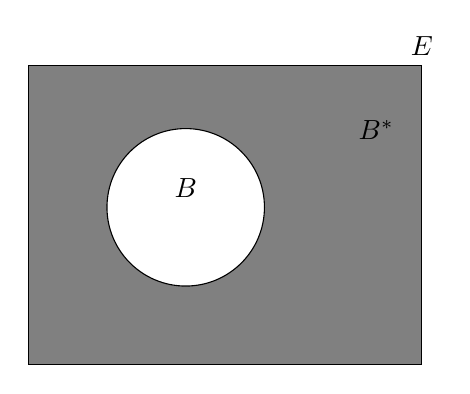
\begin{tikzpicture}
        \filldraw[fill=gray] (-2,-2) rectangle (3,1.8) node [text=black,above] {$E$} node at (19:3) [text= black, left = 2pt] {$B^*$};
        \scope % B
        \clip (0,0) circle (1);
        \fill[white] (0,0) circle (1.5);
        \endscope
        \draw (0,0) circle (1) node [text=black,above] {$B$};
\end{tikzpicture}
    \caption{Venn diagram showing a basis $B \in \mathcal B(M)$ of $M$, and a basis $B^* \in \mathcal B(M^*)$ of it's dual}%
\label{graphic}%
\end{figure}

We will consider the matroid depicted in previous sections (figure (\ref{fig:1234-matroid-circuits})). We also consider it's dual (figure (\ref{DoubleDiagramDual})). To the \textbf{left} we have the depiction corresponding to the \textbf{original matroid}, and to the \textbf{right} we have the one corresponding to its \textbf{dual matroid}. 
We notice the ground set is composed of 4 components $E=\{1,2,3,4\}$, and the original matroid has bases $12$ and $23$ (highlighed in red). Its dual has bases $34$ and $14$ respectively (also highlighted in red). This is because the complement of the elements $12$ is $34$, and the complement of $23$ is $14$.

\begin{figure}[H]
\begin{tikzpicture}[H]
\centering
\matrix (a) [matrix of math nodes, column sep=0.3cm, row sep=0.35cm,]{
 & & &\textcolor{cyan}{
1234} & & & &\\
 \textcolor{cyan}{
123}& &\textcolor{cyan}{
124} & &\textcolor{cyan}{
134} &  & \textcolor{cyan}{
234}  \\
\textcolor{red}{12} & \textcolor{blue}{13} & \textcolor{cyan}{14} & & \textcolor{red}{23} & \textcolor{cyan}{
24} & \textcolor{cyan}{
34} \\
\textcolor{orange}{1}& &\textcolor{orange}{2} & & \textcolor{orange}{3}& & \textcolor{blue}{4} \\
& & & \textcolor{orange}{\emptyset} &  & & \\
&&&&&& \\};

\foreach \i/\j in {1-4/2-1, 1-4/2-3, 1-4/2-5, 1-4/2-7, 2-1/3-1, 2-1/3-2, 2-1/3-5, 2-3/3-1, 2-3/3-3, 2-3/3-6, 2-5/3-2, 2-5/3-3, 2-5/3-7, 2-7/3-5, 2-7/3-6, 2-7/3-7, 3-1/4-1, 3-1/4-3, 3-2/4-1, 3-2/4-5, 3-3/4-1, 3-3/4-7, 3-5/4-3, 3-5/4-5, 3-6/4-3, 3-6/4-7, 3-7/4-7, 3-7/4-5, 4-1/5-4, 4-3/5-4, 4-5/5-4, 4-7/5-4}
\draw[double, line width = 0.005mm, color = brown] (a-\i) -- (a-\j);
\end{tikzpicture}
\begin{tikzpicture}[H]
\centering
\matrix (a) [matrix of math nodes, column sep=0.3cm, row sep=0.35cm,]{
 & & &\textcolor{cyan}{
1234} & & & &\\
 \textcolor{cyan}{
123}& &\textcolor{cyan}{
124} & &\textcolor{cyan}{
134} &  & \textcolor{cyan}{
234}  \\
\textcolor{cyan}{12} & \textcolor{blue}{13} & \textcolor{red}{14} & & \textcolor{cyan}{23} & \textcolor{cyan}{
24} & \textcolor{red}{
34} \\
\textcolor{orange}{1}& &\textcolor{blue}{2} & & \textcolor{orange}{3}& & \textcolor{orange}{4} \\
& & & \textcolor{orange}{\emptyset} &  & & \\
&&&&&& \\};

\foreach \i/\j in {1-4/2-1, 1-4/2-3, 1-4/2-5, 1-4/2-7, 2-1/3-1, 2-1/3-2, 2-1/3-5, 2-3/3-1, 2-3/3-3, 2-3/3-6, 2-5/3-2, 2-5/3-3, 2-5/3-7, 2-7/3-5, 2-7/3-6, 2-7/3-7, 3-1/4-1, 3-1/4-3, 3-2/4-1, 3-2/4-5, 3-3/4-1, 3-3/4-7, 3-5/4-3, 3-5/4-5, 3-6/4-3, 3-6/4-7, 3-7/4-7, 3-7/4-5, 4-1/5-4, 4-3/5-4, 4-5/5-4, 4-7/5-4}
\draw[double, line width = 0.005mm, color = brown] (a-\i) -- (a-\j);
\end{tikzpicture}

\begin{center}
\begin{tikzpicture}[H]
\centering
\node[draw] at (0, -1.5){\small \textcolor{orange}{Independent set}, \textcolor{red}{Basis}, \textcolor{blue}{Circuit}, \textcolor{cyan}{Dependent set}};

\end{tikzpicture}
\end{center}
\caption{Diagram of a 4-element matroid and its corresponding dual.}
\label{DoubleDiagramDual}
\end{figure}

% We know that the basis set of a matroid is obtained from its set of independent sets $I$.
% Using this diagrams, we highlight an idea that will be useful later in this chapter.
% That is, that the basis set of a matroid is given by a subset of $E$, the remaining elements in $E$ that are not in the basis if added to it will be linearly dependent. Aditionally we can take any remaining element of $E$ and exchange it with an element in the basis, and end up with another basis for $E$. With this intuition in mind, we can continue with a theorem.


We can formalize the definition of $\mathcal{B}^*$ and use it to construct the definition of the dual matroid.

\begin{theorem}\label{dualbasis}
    Let $M$ be a matroid given by $(E,\mathcal{B})$, and $\mathcal{B}^*(M)$ be $\{E(M) - B|B\in \mathcal{B}(M)\}$. Then $\mathcal{B}^*(M)$ is the set of bases of a matroid on $E(M)$.
\end{theorem}

\begin{defn}
     The matroid that satisfies theroem (\ref{dualbasis}), i.e., whose ground set is $E(M)$ and whose set of basis is $\mathcal{B}^*(M)$, is called the dual of M, and is denoted by $M^*$
\end{defn}

In Theorem (\ref{dualbasis}) we say that $\mathcal{B}^*(M)$ is the set of bases of a matroid on $E(M)$, but this may not be trivially clear, so we need to prove it. However, to prove it we make use of an equivalent property, which we will refer to as (B2)$^*$ (The idea to take this approach was motivated by \cite[p. 64]{oxley1}). This property comes from our property (B2) in Section 2.2 (theorem (\ref{thm:basis-properties})).

\begin{lemma}[(B2)$^*$]\label{B2Dual}
    Let $\mathcal{B}$ be the set of bases of some matroid $M$. If $B_1, B_2 \in \mathcal{B}$ and $x \in B_2 - B_1$,then there exists an element $y$ of $B_1 - B_2$ such that $(B_1 - y) \cup x \in \mathcal{B}$
\end{lemma}

For comparison, the original statement of (B2) is the following:
\begin{enumerate}
    \item[(B2)] \textit{If $B_1,B_2\in \mathcal{B}$ and $x\in B_1 - B_2$, then there exists some $y\in B_2 - B_1$ such that $(B_1 - x)\cup y \in \mathcal{B}$}.
\end{enumerate}

\begin{proof}[Proof of lemma (\ref{B2Dual})]
Assume $B_1$ and $B_2 \in \mathcal{B}$ and $x \in B_2 - B_1$.

    We note that $B_1$ is by definition a basis. This means that adding any element $x \not\in B _1 $ to $B _1 $ introduces an unique circuit $C_1 \in \mathcal{C}$ (if this circuit is not unique, and some other circuit $C _2 $ exists, we can apply (C3) to create a circuit $C _3 \subseteq C _1 \cup C _2 - x \subseteq B_1$, which would be a contradiction). Since $C_1$ is dependent and $B_2$ is independent, then $C_1 - B_2$ will be non-empty (otherwise we would have $C _1 - B _2 = \emptyset$ which implies that $C _1 \subseteq B _2$, which is a contradiction, as independent sets cannot contain dependent sets). This implies that there exists an element $y$ such that $y \in C_1 - B_2$, but as $C_1$ is the circuit created from $B_1 \cup x$, then $y \in (B_1 \cup x) - B_2$. Similarly, as $x \neq y$ (because $x \in B _2 $ and $y \not\in B _2$), then $y \in B_1 - B_2$. 

    Consider the set $B_1 - y$. This will not be a basis (because all bases have equal cardinality), but it will be an independent set (implied by (I2)). We notice that $(B_1 - y)\cup x$ will clearly not contain the circuit $C_1$, since $y \in C _1 $ and $y \not\in (B _1 - y) \cup x$. Furthermore, this set cannot contain any other distinct circuit $C _2 \in \mathcal{C}$, because that would imply $C _2 \subseteq B _1 \cup x$, which would contradict the uniqueness of $C _1 $. We can now conclude that the set $(B_1 - y)\cup x$ must be independent. We observe that $(B_1 - y)\cup x$ implies that we add an element to the set, and we take out one element of the set, so the cardinality will remain equal, that is: $|(B_1 - y)\cup x|=|B_1|$.

As $(B_1 - y)\cup x$ is independent and has the same cardinality as the basis $B_1$, then by definition $(B_1 - y)\cup x$ is also a basis. 
\end{proof}

Now, using the equivalent property $(B2)^*$ that we have just proven, we prove theorem (\ref{dualbasis}).
\begin{proof}[Proof of (\ref{dualbasis})]
    As $\mathcal{B}(M)$ is non-empty, $\mathcal{B}^*(M)$ is non-empty, hence, the property $(B_1)$ holds for $\mathcal{B}^*(M)$. 
    Consider two distinct members $B^* _1 , B ^* _2 \in \mathcal{B}^*(M)$, such that there exists an element $x \in (B^*_1 - B^*_2)$. Let, $B_1 = E - B^*_1$ and $B_2 = E - B^*_2$. We can see that $B^*_1 - B^*_2 = B_2 - B_1$, thus $x \in B_2 - B_1$. By ${(B2)}^*$, there exists and element $y \in  B_1 - B_2$ such that $(B_1 - y)\cup x$ is a base of $M$, but observe that $B_1 - B_2 = B^*_2 - B^*_1$, so this is the same as saying that there exists an element $y \in  B^*_2 - B^*_1$ such that $(B_1 - y)\cup x$ is a base of $M$. As a result, by definition of the dual, $E-((B_1 - y)\cup x) \in \mathcal{B}^*(M)$. But, $E-((B_1 - y)\cup x) = ((E-B_1)-x)\cup y) = (B_1^* - x)\cup y$, which is in the family $\mathcal{B}^*$. Therefore, we can conclude that $B^*(M)$ satisfes $(B2)$. As $\mathcal{B}^*(M)$ satisfies  properties $(B1)$ and $(B2)$, this is indeed the set of bases of a matroid on $E$.
\end{proof}

Note that, by the way the dual matroid is defined, and and by the intuition provided in the proof above, we see that $\mathcal{B}(M^*)=\mathcal{B}^*(M)$. Furthermore, we have the following lemma:

\begin{lemma}
    The dual of the dual of a matroid M is the matroid M itself, $i.e., (M^*)^* = M$.
\end{lemma}

This is because if we take the complement $B^*$ of the basis set $B$, and then we take this complement $B^*$ and take its complement once again, we will return to the original set $B$. In other words:
\begin{align*}
E-(E - B) = B.
\end{align*}

\begin{exmp}
    Let $U_{k,n}$, be a uniform matroid. We know that its bases will be all the k-element subsets of $E(U_{k,n})$. We also know, by definition (\ref{uniformM}), that this matroid is defined over a set of $n$ elements, and its basis has exactly $k$ elements. Therefore, the bases of $U_{k,n}$* are all $(n-k)-element$ subsets of the ground set, as this will be the complement of the basis set of $U_{k,n}$. This is equal to saying that the dual of the matroid $U_{k,n}$ is given by 
    \begin{align*}
    U_{k,n} ^*  = U_{n-k,n}.
    \end{align*}
\end{exmp}

Now that we have introduced the notion of duals, it is useful to provide some additional notation. That is, given a matroid $M$ with a dual $M^*$, the \textit{bases} of the matroid $M^*$ are called \textit{cobases} of $M$. Similarly, the \textit{independent sets} of $M^*$ are called \textit{coindependent sets} of $M$, the $circuits$ of $M^*$ are called \textit{cocircuits} of $M$, \textit{hyperplanes} (see definition (\ref{HP&SS})) are called \textit{cohyperplanes}, and the \textit{spanning sets} (see definition (\ref{HP&SS})) are called \textit{cospanning sets} of $M$ and so on. This leads us to some elementary relationships between these sets. 

\begin{theorem}\label{propositionsofdualrelations}
    Let M be a matroid in a set E and suppose $X \subseteq E$. Then,
    \begin{enumerate}
        \item $X$ is independent if and only if $E-X$ is cospanning.
        \item $X$ is spanning if and only if $E-X$ is coindependent.
        \item $X$ is a hyperplane if and only if $E-X$ is a cocircuit
        \item $X$ is a circuit if and only if $E-X$ is a cohyperplane.
    \end{enumerate}
\end{theorem} 

\begin{proof}
    Let us prove theorem (\ref{propositionsofdualrelations}). All of the proofs follow directly from the definitions.

    \begin{enumerate}
        \item  \begin{enumerate}
            \item[$\implies$] Suppose $X$ is independent. This means there exists a basis $B \in \mathcal{B}(M)$ so that $X \subseteq B$. Because $X \subseteq B \subseteq E$ and the operation of taking complements is ``inclusion reversing" we have $E-B \subseteq E - X$. Verifying directly, if $x \in E - B$ this means $x \in E$ and $x \notin B$. Because $X \subseteq B$ this implies that $x \in E$ and $x \notin X$ so by definition $x \in E - X$ and the conclusion follows. Because $E - B$ is a cobasis and $E - X$ is a set containing a cobasis, then it is a cospanning by definition.
            \item[$\impliedby$] Similarly if $E - X$ is cospanning then it contains a cobasis which is by definition of the form $E - B$ for some $B \in \mathcal{B}(M)$. By the analogous reasoning as for the forward direction $E - B \subseteq E - X$ implies $X \subseteq B$. That is because if $x \in X$ then $x \notin E - X$ and $x \notin X - B$. This means $x \in B$ concluding $X \in B$. Since $B$ is an independent set then $X$ is an independent set as well, we are done.
        \end{enumerate}

   \item  \begin{enumerate}
    \item[$\implies$] A set $X\subseteq E$ being spanning implies it contains a $B \in \mathcal{B}(M)$. So  $B \subseteq X$ which implies $E - X \subseteq E - B$. Because $E - B$ is cobasis by definition, any of its subsets are coindependent. 
    \item[$\impliedby$] If $E - X$ is coindependent, it is contained in a cobasis, so by definition there exists a $B \in \mathcal{B}$ so that $E - X \subseteq E - B$. As before this implies that $B \subseteq X$ and $X$ is spanning.
   \end{enumerate}

    \item  \begin{enumerate}
        \item[$\implies$] If $X$ is a hyperplane, then $X$ is not spanning, but for all $y \in E - X$ we have $X \cup y$ is spanning, which means there is for every such $y$ a basis $B_y \in \mathcal{B}$ so that $B_y \subseteq X \cup y $. By b) we know that $X$ is not spanning implies $E - X$ is not coindependent. But for any $z \in E - X$ we have $(E-X)-z = E - (X \cup z)$ is coindependent because $X \cup z$ is spanning. So $E - X$ is a cocircuit by definition.
        \item[$\impliedby$] Conversly, if $E - X$ is a cocircuit, then $E-X$ is not coindependent but for all $x \in E - X$ we have $(E - X) - x$ = $E - (X \cup x)$ is coindependent. By b) this means that $X$ is not spanning but for all $x \in E-X$, we have $X \cup x$ is spanning, so $X$ is a hyperplane.
    \end{enumerate}

\item The proof is completely analogous to the previous ones. \qedhere
    \end{enumerate}
\end{proof}

Similar to bases and cobases, the $rank$ $ function$ of the dual matroid is usually denoted by $r^*$, and is normally referred as the \textit{corank function} of $M$. Using the definition of bases of the dual matroid, as well as the fact that a matroid and its dual have the same ground set, we have the following

\begin{theorem}\label{RankAndCorankEquation}
  The following equality holds  $r(M) + r^*(M) = |E(M)|=|E(M^*)|$.
\end{theorem}

In fact, we can generalize the above theorem to obtain an explicit formula for the \textit{corank function} of the matroid. 

\begin{theorem}\label{rankdualequation}
    For all subsets $X \subseteq E(M)$ of some matroid $M$, we have:
    \begin{align*}
    r^*(X)=r(E-X)+|X|-r(M)
    \end{align*}
\end{theorem}

\begin{proof}[Proof of theorem (\ref{rankdualequation})]
    Let $I^* \subseteq X$ be an independent subset of $X$ in $M^*$, such that it is not a subset of some other set in $X$. That is, $r^*(X)=|I^*|$. Similarly, let $I$ be an independent subset of $E-X$ in $M$, such that it is not a subset of some other set in $E-X$. That is, $r(E-X)=|I|$. Let $B$ be an independent subset of $E-I^*$, such that it is not a subset of some other set in $E-I^*$ and contains $I$. Since, these are independent subsets that are not subsets of any other element in their respective sets, then we have $r(B)=r(E-I^*)$ and $r(E-I^*)=r(M)$, and hence $B$ is a basis of $M$.
    Let $B^*=E-B$. Since $B$ is a basis of $M$, then $B ^* $ is also a basis of $M^*$. We observe that $I^*\subseteq B^*$ and  $B^*\cap X=I^*$. Similarly, $I\subseteq B$ and  $B\cap (E-X)=I$. In particular, we see that, $|B\cap X|=|B|-|I|$, thus
    \begin{align*}
    |X|=|X\cap B|+|X\cap B^*|=|B|-|I|+|I^*|=r(M)-r(E-X)+r^*(X).
    \end{align*}
    \qedhere

\end{proof}

\newpage
\subsection{Duals of representable matroids}

Let $A\in \mat_{m\times n}(\mathbb{F})$, and let $M$ be a vector matroid $M[A]$ of $A$. The ground set of $M$ is then the set $E$ of column labels of $A$. Note that, in general, $M[A]$ does not uniquely determine $A$. Furthermore, $M$ remains unchanged if we perform any of the following operations on $A$, which includes the \textit{elementary row operations}.
\begin{enumerate}
    \item Interchange two rows.
    \item Multiply a row by a non-zero member of $\mathbb{F}$.
    \item Replace a row by the sum of that row with another row.
    \item Ad or remove a zero row.
    \item Interchanging two columns (the labels moving with the columns).
    \item Multiply a column by a non-zero member of $\mathbb{F}$.
\end{enumerate}

The reason for this is that when constructing the matroid $M$ from a matrix $A$, we only care about the independence (or dependence) between column vectors in the matrix. As long as the independence and dependence between them is kept the same, the exact values inside the columns are not relevant.

Assume that $A$ is non-zero. It is easy to prove that by using the previously mentioned operations, $A$ can be reduced to be of the form $[I_r|D]$, where $I_r$ is the $r \times r$ identity matrix ($1\leq r< n$) and $D$ is some $r \times (n-r)$ matrix over $\mathbb{F}$. This is because using the \textit{elementary row operations} we can reduce the matrix $A$ to its \textit{reduced row echelon form} and then using the remaining operations we can remove any zero row (operation 4.) and interchange any columns to make sure is in the desired from (operation 5.). We also can clearly see that $r(M)=r$ (the dimension for the identity matrix). 

Suppose the columns of $[I_r|D]$ are labelled as $e_1, e_2,\cdots,e_n$. We then have the ground set $E=\{e_1, e_2,\cdots,e_n\}$. Let, $\{e_1, e_2,\cdots,e_r\}$ be a basis $B$ of $M$. We also label the rows and columns of the submatrix $D$ in the following form:
\begin{itemize}
  \item We label the rows from top to bottom as $e_1, e_2,\cdots,e_r$.
  \item We label the columns as left to right $e_{r+1}, e_{r+2},\cdots,e_n$.
\end{itemize}

  This way to represent $M[A]$ can be seen more clearly in figure (\ref{StandertRepMat}). We will refer to both $[I_r|D]$ and $D$ as the \textit{standard representative matrices} for $M$, \textit{with respect to $\{e_1, e_2,\cdots,e_r\}$}. Similarly, we use \textit{reduced standard representative matrix} if we want to refer only to $D$.

\begin{figure}[H]
    \centering
    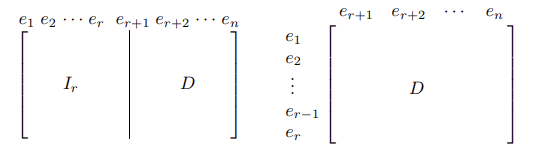
\includegraphics{SRF.png}
    \caption{Standard representative matrices for $M$ (Taken from \cite[p. 78]{oxley1}).}
    \label{StandertRepMat}
\end{figure}

Note that in the matrix $[I_r|D]$ from figure (\ref{StandertRepMat}),  only the columns are labelled, but in $D$, both the rows and columns ae labelled. Also note that, for the basis $B=\{e_1, e_2,\cdots,e_r\}$ of $M$ defined in figure (\ref{StandertRepMat}), the columns correspond to the columns of the identity matrix.

We can now use this construction to determine the dual of a vector matroid using the following theorem

\begin{theorem}\label{DualRepMat}
    Let M be the vector matroid of the matrix $[I_r|D]$ where the columns are labelled, in order $e_1, e_2,\cdots,e_n$ and $1\leq r< n$. Then $M^*$ is the vector matroid of $[-D^T|I_{n-r}]$, where its columns are also labelled $e_1, e_2,\cdots,e_n$ in that order.
\end{theorem}

The following proof was inspired by that in \cite[p. 78]{oxley1}.

\begin{proof}
    We assume that $[I_r|D]$ is as in the contruction of the theorem above. Then $[-D^T|I_{n-r}]$ is as shown in figure (\ref{MatRepresentationDual}).
    \begin{figure}[h]
        \centering
        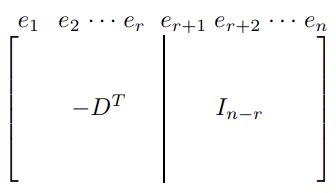
\includegraphics{VMRDual.png}
        \caption{Standart representative form of the dual of a matroid as established in theorem (\ref{DualRepMat}) ((Taken from \cite[p. 78]{oxley1}).}
        \label{MatRepresentationDual}
    \end{figure}

    Let $B$ be a basis of $M$. We need to show that $E-B$ is a basis of the vector matroid of $[-D^T|I_{n-r}]$. We can rearrange the columns of $[-D^T|I_{n-r}]$, such that $B=\{e_1,\cdots,e_s, e_{r+1}, \cdots, e_{r+(r-s)}$\}, for some $s \leq r$. This is possible because we know that it does not affect the corresponding matroid since we are only doing the elementary row operations. Therefore the only change it bring to rearrange rows and columns of $[I_r|D]$ is the rearrange of columns and rows of $[-D^T|I_{n-r}]$. 
    
    Using this, we can partition $[I_r|D]$ and $[-D^T|I_{n-r}]$ in the following form
    \begin{align*}
    \begin{bmatrix}
    I_s & 0 & D_{11} & D_{12}\\
    0 & I_{r-s} & D_{21} & D_{22}\\.
    \end{bmatrix}
    % 
         \rightarrow 
    \begin{bmatrix}
    -D_{11}^T & -D_{21}^T & I_{r-s} & 0\\
    -D_{12}^T & -D_{22}^T & 0 & I_{n-(2r-s)}\\
    \end{bmatrix}
    \end{align*}
    We will analyze the way $[I_r|D]$ is partitioned. Here, we make the partitioning such that the first component $I_s$ has columns $(e_1 \cdots e_s)$, $I_{r-s}$ has columns $(e_{s+1} \cdots e_r)$, $D_{11}$ and $D_{21}$ have columns $(e_{r+1} \cdots e_{2r-s})$, and finally, $D_{12}$ and $D_{22}$ have columns $(e_{(2r-s)+1} \cdots e_n)$.
    
    We have that $B$ is a base. This means that it must have the same size as $I_r$. Due to the way the matrix $[I_r|D]$ is partitioned, if we take the components in the partition that contain the column components in the basis, we get the following matrix
        \begin{align*}
        \begin{bmatrix}
        I_s & D_{11}\\
        0 & D_{21}\\
        \end{bmatrix}.
        \end{align*}

    As this matrix has the partition components that contain all the elements in the basis, it must have a $rank$ of $r$ (the $rank$ of $[I_r|D]$). Here $r(I_s) = s$, as it is the identity matrix, hence $r(D_{21})=r-s$, which also corresponds to the rank of $-D_21^T$.
    
    If we now observe the partition of $[-D^T|I_{n-r}]$, this will give the same partition lengths in each component as the ones mentioned for $[I_r|D]$ above. That is, the first component $-D_{11}^T$ and $-D_{12}^T$ have columns $(e_1 \cdots e_s)$. The components $-D_{22}^T$ and $-D_{21}^T$ have columns $(e_{s+1} \cdots e_r)$, $I_{r-s}$ has columns $(e_{r+1} \cdots e_{2r-s})$, and finally $ I_{n-(2r-s)}$ has columns $(e_{(2r-s)+1} \cdots e_n)$.

    As this time we are dealing with the dual, instead of taking the components that contain the elements in the basis like before, we take the components in the partition of $[-D^T|I_{n-r}]$ that contain the complement of the elements in the basis. Therefore, we obtain the matrix
    \begin{align*}
        \begin{bmatrix}
        -D_{21}^T & 0\\
        -D_{22}^T & I_{n-(2r-s)}\\
        \end{bmatrix}.
    \end{align*}

   The rank of this submatrix is the sum of the ranks of $I_{n-(2r-s)}$ and $-D_{21}^T$. We have previously stated that the rank of $-D_{21}^T$ is the same as the one of $D_{21}$. That is, $r(-D_{21}^T)= r-s$, and the $rank$ of $I_{n-(2r-s)}$ is $n-(2r-s)$, which means the total rank is 
   \begin{align*}
    (r-s)+(n-(2r-s))= r-s+n-2r+s = n-r.
   \end{align*}

    This implies that $E-B$ is a basis of the vector matroid of $[-D^T|I_{n-r}]$, since $|E|= n$ and $|B|= r$. This corresponds to the definition of the dual, whose basis $B^*$ must satisfy $|B^*|= n-r$, which holds in this case. This argument could be easily extended to show that every basis of the matroid appears in this way. Therefore, $[-D^T|I_{n-r}]$ is indeed a representation of $M^*$.
\end{proof}

By convention, the form $[-D^T |I_{n-r}]$ is used instead of $[D^T |I_{n-r}]$. However, it is important to remark that this does not bring any issues, because the use of \textit{elementary row operations} does not affect the matroid of a matrix. 

A remarkable result follows almost directly from theorem (\ref{DualRepMat}):

\begin{corollary} \label{corollaryrepdual}
    If a matroid $M$ is \textit{representable} over a field $\mathbb{F}$, then $M ^* $ is also representable over the same field $\mathbb{F}$.
\end{corollary}

\begin{proof}
    Let us prove the Corollary above. Suppose we have a matroid $M$ with rank $m$. That is, the bases of $M$ have size $m$. Then, by assumption, we can say (without loss of generality) that $M$ can be represented by some $m \times n$ matrix $H$ (with $1\leq n < m$), such that $H=[I_{m}|D_{m \times (n-m)}]$ over $\mathbb{F}$. By theorem (\ref{DualRepMat}), its dual is then represented by 
    \begin{align*}
    H^*=[-D^T|I_{(n-m) \times (n-m)}]=[-D_{(n-m) \times m}|I_{(n-m)}],
    \end{align*}
    which is also a matrix over $\mathbb{F}$.
\end{proof}

\begin{exmp}
    Consider the vector matroid $M$ with the following representation over $\mathbb{R}$
    \begin{align*}
        A = \begin{bmatrix}
            1 & 0 & 0 & 1 & 0 & 1 \\
            0 & 1 & 0 & 1 & -1 & 0 \\
            0 & 0 & 1 & 0 & 1 & 1 \\
        \end{bmatrix}.
    \end{align*}

Then, by theorem (\ref{DualRepMat}), the corresponding dual matroid $M^*$ is the vector matroid represented by 
\begin{align*}
        A^* = \begin{bmatrix}
            -1 & -1 & 0 & 1 & 0 & 0 \\
            0 & 1 & -1 & 0 & 1 & 0 \\
            -1 & 0 & -1 & 0 & 0 & 1 \\
        \end{bmatrix}.
\end{align*}

As an interesting note, the vector matroid $M$ with matrix representation $A$ is associated to the graph $K_4$. In other words, this means that the matrix $A$ and the graph $K_4$ (figure (\ref{K4Graph})) produce the same matroid.

       \begin{figure}[H]
        \centering
            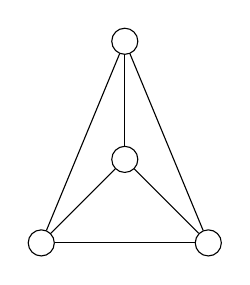
\begin{tikzpicture}[
                node distance = 15mm and 15mm,
                V/.style = {circle, draw, fill=white!30},
                every edge quotes/.style = {auto, font=\footnotesize, sloped}
                    ]
                \begin{scope}[nodes=V]
                \node (1) {}; 
                \node (2) [below of=1] {}; 
                \node (3) [below left of=2] {}; 
                \node (4) [below right of=2] {}; 
                \end{scope}
                \draw (1) to (2); 
                \draw (1) to (3);
                \draw (1) to (4); 
                \draw (2) to (3);
                \draw (2) to (4); 
                \draw (3) to (4);
            \end{tikzpicture}
            \caption{$K_4$, the complete graph on 4 vertices.}
            \label{K4Graph}
        \end{figure}

    Additionally, we can also verify the \textit{rank} and \textit{corank} propositions established before (theorem (\ref{RankAndCorankEquation})). That is, we can clearly observe that $A$ has a ground set $E=\{e_1, e_2, \cdots, e_6\}$ with $6$ elements, where each $e_i; i =1,2, \cdots,6$ represents a column, hence $|E|=6$. We also see that $A$ has rank $r(A)=3$, which can be easily verified by observing the first $3$ columns that correspond to the identity matrix in the construction of the form $[I_r|D]$. Similarly, if we observe the dual, we notice that $r(A^*)=3$ as well. We conclude that 
    \begin{align*}
    r(A)+r(A^*)= 3 + 3 = 6 = |E|.
    \end{align*}
\end{exmp}

%

\subsection{Dual of graphic matroids}
We have studied many concepts related to dual matroids, including some representations for vector matroids. We have however not gone into detail with regard to graphic matroids. We then pose the question --- \textit{``Is it possible to have a graphic matroid whose dual is not graphic?"}

To answer this question, we have the following theorem

\begin{theorem}
    The dual of a graphic matroid is itself graphic if and only if the underlying graph is planar.
\end{theorem}

The proof for this theorem is outside the scope of this article. A proof can be found in \cite[p. 140, section 5.2]{oxley1}.

\begin{exmp}
    Let us consider the bipartite graph $K_{3,3}$.
\begin{figure}[H]
\centering
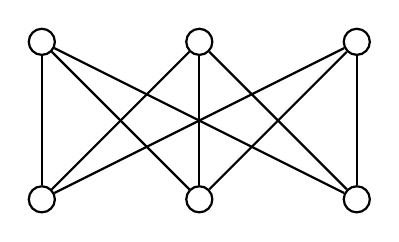
\begin{tikzpicture}[node distance={20mm}, thick, main/.style = {draw, circle}] 
    \node[main] (1) {}; 
    \node[main] (2) [below of=1] {}; 
    \node[main] (3) [right of=1] {}; 
    \node[main] (4) [below of=3] {}; 
    \node[main] (5) [right of=3] {}; 
    \node[main] (6) [below of=5] {}; 
    \draw (1) to (2); 
    \draw (1) to (4);
    \draw (1) to (6); 
    \draw (3) to (2);
    \draw (3) to (4); 
    \draw (3) to (6);
    \draw (5) to (2); 
    \draw (5) to (4);
    \draw (5) to (6);
    \end{tikzpicture}
    \caption{The bipartite graph $K_{3,3}$}
    \label{fig:enter-label}
\end{figure}

This graph has $9$ edges, which means it has $E=\{1,2,3, \cdots, 9\} $ as its ground set. The matrix associated to the matroid $M(K_{3,3})$ is the following:
\begin{align*}
J = \begin{bmatrix}
    1 & 0 & 0 & 0 & 0 & 1 & 0 & 0 & 1\\
    0 & 1 & 0 & 0 & 0 & 1 & 1 & 0 & 1\\
    0 & 0 & 1 & 0 & 0 & 1 & 1 & 1 & 1\\
    0 & 0 & 0 & 1 & 0 & 0 & 1 & 1 & 1\\
    0 & 0 & 0 & 0 & 1 & 0 & 0 & 1 & 1\\
\end{bmatrix}.
\end{align*}

    This is the case because labelling the columns of $J$ as $E = \{e_1,\cdots, e_9\}$ and defining a matroid $M(J)$ on $E$, lets us associate each column of $J$ to the correspondingly labeled edge in $K_{3,3}$ and we can directly verify that they represent the same matroid (the matroids are isomorphic). Moreover, this means that we can take a basis for the column space of $J$, such as $B = \{e_1, e_2, e_3, e_4, e_5\}$, that corresponds to a spanning tree $T$ of $K_{3,3}$ (see figure (\ref{K33STE})). In other words, this means that adding any other column to $J$ yields a linear dependency (more precisely, a circuit in $M(J)$), and adding any edge to $T$ generates a cycle.

\begin{figure}[H]
    \centering
    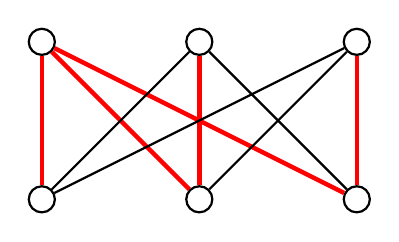
\begin{tikzpicture}[node distance={20mm}, thick, main/.style = {draw, circle}] 
        \node[main] (1) {}; 
        \node[main] (2) [below of=1] {}; 
        \node[main] (3) [right of=1] {}; 
        \node[main] (4) [below of=3] {}; 
        \node[main] (5) [right of=3] {}; 
        \node[main] (6) [below of=5] {}; 
        \draw [ultra thick,red] (1) to (2); 
        \draw [ultra thick,red] (1) to (4);
        \draw [ultra thick,red] (1) to (6); 
        \draw (3) to (2);
        \draw [ultra thick,red] (3) to (4); 
        \draw (3) to (6);
        \draw (5) to (2); 
        \draw (5) to (4);
        \draw [ultra thick,red] (5) to (6);
    \end{tikzpicture}
    \caption{Graph $K_{3,3}$, showing in red an example of edges that form a spanning tree, that can be associated accordingly to the basis of $J$.}
    \label{K33STE}
\end{figure}

Now that we have show that $K_{3,3}$ has an associated matrix, which produces the same matroid, we can use theorem (\ref{DualRepMat}) to obtain the corresponding dual:
\begin{align*}
  J^*=\begin{bmatrix} 
1 & 1 & 1 & 0 & 0 & 1 & 0 & 0 & 0\\
0 & 1 & 1 & 1 & 0 & 0 & 1 & 0 & 0\\
0 & 0 & 1 & 1 & 1 & 0 & 0 & 1 & 0\\
1 & 1 & 1 & 1 & 1 & 0 & 0 & 0 & 1\\
\end{bmatrix}
\end{align*}

As a sanity check, we can see that $r(J) = 5$,  $r^*(J)=4$, and $|E(M)|=9$. We then notice the following does indeed hold:
\begin{align*}
r(M) + r^*(M) = |E(M)|.
\end{align*}

According to corollary (\ref{corollaryrepdual}), \textit{If a matroid \textit{M} is \textit{representable} over a field $\mathbb{F}$, then \textit{M*} is also representable over $\mathbb{F}$}. Here we see that both matroids are vector matroids over the field $\mathbb{F}_2$. 

Finally, we can observe that $K_{3,3}$ is not a planar graph. This implies that, although $M(K_{3,3})$ is a graphic matroid, its dual ($M^*(K_{3,3})$) is not graphic.
\end{exmp}

\newpage
\section{Conclusion}
In the article, we discussed several equivalent definitions of matroids. As a starting point, we choose the definition in terms of independent sets. We saw they naturally abstract the linear independent subsets of vector spaces. We then proceeded by showing the description in terms of maximal independent sets - bases. Afterward we moved to circuits and how they can, in one hand, be interpreted as minimal dependent, or on the other, as object naturally abstracting graphic cycles. We then moved on to more intricate objects, which described the matroid by assigning some value to each set. First we saw the rank function and second the closure operator, both providing a new perspective on how to describe the matroids by not listing subsets directly, but rather present it using a function. Lastly, we introduced the concept of flat. Along the way, we proved the cryptomorphism - that is, that the matroid can be described starting from any viewpoint. As an example, we showed that the algebraically dependent sets in field extensions also have a natural matroid structure, even though the matroid modeled a much broader concept of algebraic independence and no longer linear independence. As our last illustration of matroids we turned away from cryptomorphisms and defined the concept of a matroid dual which had many interesting new properties, and also extended the existing ones, such as it was the case with the corank function, coindependent sets, cobases and cocircuits. Finally, we showed that it is possible for the dual of a graphic matroid to be non-graphic.


\appendix
\subsection{Fields}\label{sec:appendix-fields}

This section provides a basic introduction to working with fields. For a more formal in depth treatment of the topic, check~\cite{milne2022}.

\begin{defn}[Fields]
  Intuitively, a field is a triplet consisting of a set and two binary operations, which are usually referred to as addition and multiplication. Both these operations are associative, commutative, and have identity elements (usually referred to as $0$ and $1$ respectively). All elements have inverse elements for addition. Similarly, all nonzero elements have inverses for multiplication. Furthermore, the two operations obey distributivity laws.
\end{defn}

\begin{defn}[Subfields]
  Intuitively, given a field $K$, a subfield is a subset $F \subseteq K$ together with restrictions of addition and multiplication to $F$. Formally, the following three properties must hold:
  \begin{enumerate}
    \item $1 \in F$
    \item $a, b \in F \implies a - b \in F$
    \item $a, b \in F \;\text{and}\; b \neq 0\implies a b ^{-1}  \in F$
  \end{enumerate}
\end{defn}

\begin{defn}[Algebraic elements]
  Given a field $K$ and a subfield $F$, an element $a \in K$ is said to be algebraic over $F$ if there exists a nonzero polynomial $f$ with coefficients in $F$ such that $f(a) = 0$. Elements which are not algebraic are said to be transcendental.
\end{defn}


Throughout \hyperref[sec:algebraic-matroids]{the section on algebraic matroids} we use the notation $F[X _1 \ldots X_n]$ to refer to the set of polynomials with $n$ variables and coefficients in some field $F$. This set presents a ring structure, but understanding that is not necessary for understanding this article. A more in depth treatment of polynomial rings can be found in~\cite{milne2022}.


\begin{defn}[Adjoining elements to a field] \label{def:field-adjoint}
  Given a field $F$ and some element $e$, we can construct a new field $F(e)$ with elements of the form:
\begin{align*}
  \frac{\sum a _i e ^i }{\sum b _i e ^i },
\end{align*}
where $a _i, b _i \in F$.

  Furthermore, we will use the notation $F(a _1 ,\ldots, a _n)$ to refer to $F(a _1) \ldots (a _n)$.
\end{defn}

\newpage
\begin{exmp} \label{exp:q-adjoint-sqrt-3}
  Consider the field $\mathbb Q$  and the element $\sqrt 3$. We notice that 
  \begin{align*}
    {(\sqrt 3)} ^{2k} = 3 ^k && \text{and} && {(\sqrt 3)} ^{2k + 1} = 3 ^k \sqrt 3.
  \end{align*}

  This let us rewrite the form the elements are introduced in by definition (\ref{def:field-adjoint}) as
  \begin{align*}
    \frac{\sum a _i {(\sqrt 3)} ^i }{\sum b _i {(\sqrt 3)} ^i }
    &= \frac{\sum a _{2i} 3 ^i + \sum a_{2i + 1} 3 ^i \sqrt 3}{\sum b _{2i} 3 ^i + \sum b_{2i + 1} 3 ^i \sqrt 3} 
    \\&= \frac{a + b\sqrt 3}{c + d\sqrt 3}
    \\&= \frac{(a + b \sqrt 3)(c - d \sqrt 3)}{(c + d \sqrt 3)(c - d \sqrt 3)}
    \\&= \frac{(ac - 3bd) + (bc - da) \sqrt 3}{c ^2 - 3 d ^2 }
    \\&= \frac{ac - 3bd}{c ^2 - 3 d ^2 } + \frac{bc - da}{c ^2 - 3 d ^2 } \sqrt 3,
  \end{align*}
  where the second equality follows by choosing rationals $a, b, c, d \in \mathbb{Q}$ defined as
  \begin{align*}
    a = \sum a _{2i} 3 ^i && b = \sum a _{2i + 1} 3 ^i  &&
    c = \sum b _{2i} 3 ^i && d = \sum b _{2i + 1} 3 ^i 
  \end{align*}

  We can now define $p = \frac{ac - 3bd}{c ^2 - 3 d ^2 }$ and $q = \frac{bc - da}{c ^2 - 3 d ^2 }$ to show that all elements of $ \mathbb{Q} (\sqrt{3})$ are of the form $p + q \sqrt 3$. Moreover, it follows trivially from  definition (\ref{def:field-adjoint}) that all elements of the form $p + q \sqrt 3$ are elements of $\mathbb{Q} (\sqrt{3})$. Let $F = \{p + q \sqrt 3 \:|\: p, q \in \mathbb{Q} \}$ Having proven both 
  \begin{align*}
     F \subseteq \mathbb{Q} (\sqrt 3) && \text{and} && F \supseteq \mathbb{Q} (\sqrt 3),
  \end{align*}
 we can conclude that $\mathbb{Q} (\sqrt{3})  = F$.

  Addition will then be performed component-wise, i.e. 
  \begin{align*}
  (a + b \sqrt 3) + (c + d \sqrt 3) = (a + c)  + (b + d) \sqrt 3.
  \end{align*}

  Multiplication is a bit more involved:
  \begin{align*}
    (a + b \sqrt 3)(c + d \sqrt 3) = (ac + 3bd) + (ad + bc) \sqrt 3.
  \end{align*}

  We will now prove that $ \mathbb{Q}(\sqrt{3})$ is indeed a field, as stipulated by the definition. Associativity,  commutativity, and distributivity follow by direct computation. Similarly, $0$ and $1$ are both of the form $p + q \sqrt 3$, so both additive and multiplicative identities exist ($a + 0 = a$ and $a \cdot 1 = a$ can also be checked by direct computation). Furthermore, for any $p + q \sqrt 3$ we have $-p -q \sqrt 3$ such that 
  \begin{align*}
    p + q\sqrt 3 + (- p - q\sqrt 3) = (p - p) + (q - q) \sqrt 3 = 0.
  \end{align*}

  Similarly, if $p, q \neq 0$ we notice that $p ^2 - 3 q ^2 = 0$ holds only if $p = q \sqrt 3$, but this is never the case since $p, q \in \mathbb{Q}$. We construct $\frac p {p ^2 - 3 q ^2 } - \frac q {p ^2 - 3 q ^2 } \sqrt 3$ such that
  \begin{align*}
    (p + q \sqrt 3)\left(\frac p {p ^2 - 3 q ^2 } - \frac q {p ^2 - 3 q ^2 } \sqrt 3\right)
    &= \frac {p ^2}  {p ^2 - 3 q ^2 } - \cancel{\frac {pq} {p ^2 - 3 q ^2 } \sqrt 3}
    + \cancel{\frac {pq}  {p ^2 - 3 q ^2 } \sqrt 3} - 3\frac {q ^2 } {p ^2 - 3 q ^2 }
    \\&= \frac{p ^2 - 3 q ^2 }{p ^2 - 3 q ^2 }
    \\&= 1.
  \end{align*}

  We can now conclude that all elements have additive inverses, and that all nonzero elements have multiplicative inverses. This, together with the previously proven properties, let us conclude that $\mathbb{Q} (\sqrt{3})$ is indeed a field.
\end{exmp}

\begin{defn}[Field extensions]
 Given a field $K$ and a subfield $F$, $K$ is said to be a field extension of $F$.
\end{defn}

\begin{lemma}[Vector space structure of field extensions]\label{lem:field-extension-vector-space}
  Given a field $F$ and a field extension $K$, we can construct a vector space with elements of $F$ as scalars, elements of $K$ as vectors:
  \begin{itemize}
    \item vector addition (together with its identity element and inverse) is defined the same way as addition in $K$. 
    \item scalar-vector multiplication (together with its identity element and inverse) is defined the same way as multiplication in $K$ (because all scalars are also vectors, since elements of $F$ are also elements of $K$).
    \item scalar-scalar multiplication (together with its identity element and inverse) is defined the same way as multiplication in $F$.
  \end{itemize}
\end{lemma}

\begin{lemma}\label{lem:algebraic-field-finite-vector-space}
   Given a field $K$ and a subfield $F$, with some $a \in K$ algebraic over $F$, the vector space induced by $F(a) $ over $F$ will be finite-dimenssional.
\end{lemma}

Proving the above lemma is outside the scope of this article, but a proof can be found in~\cite{milne2022}.

\begin{exmp}
  We will study the vector space induced by $\mathbb{Q} (\sqrt 3)$ over $\mathbb{Q}$. We recall from example (\ref{exp:q-adjoint-sqrt-3}) that elements of $\mathbb{Q} (\sqrt 3)$ are of the form $p + q \sqrt 3$ where $p, q \in \mathbb{Q}$. We notice that $B = \{1, \sqrt 3\}$ forms a basis for the vector space induced by $\mathbb{Q} (\sqrt 3)$ over $\mathbb{Q} $. It's clear that $\spann B = \mathbb{Q} (\sqrt 3)$ (because for any $v = p + q \sqrt 3 \in \mathbb{Q} (\sqrt 3)$ we can pick scalars $p, q \in \mathbb{Q} $ such that $p \cdot 1 + q \cdot \sqrt 3 = v$). 

  It remains to show that $1$ and $\sqrt 3$ are linearly independent. Assume this is not the case. We now have nonzero $p, q \in \mathbb{Q} $ such that $p + q \sqrt 3 = 0$. If $q = 0$ then $p = 0$, hence a contradiction. Some simple algebraic manipulations then imply that $\sqrt 3  = \frac p {-q}$, but $\frac p {-q} \in \mathbb{Q} $ and $\sqrt 3 \not\in \mathbb{Q} $, hence another contradiction.
\end{exmp}



\nocite{*} 
\bibliographystyle{abbrv}
\bibliography{sources}


\end{document}
